\documentclass[letterpaper,twocolumn,10pt]{article}
\usepackage{usenix}
\usepackage{etoolbox}
\usepackage{xurlshawn}
% \usepackage[hyphenbreaks]{breakurl}

\makeatletter
\patchcmd{\maketitle}
  {\@maketitle}
  {\vspace{-0.3in}\@maketitle\vspace{-0.4in}}% change the value as needed
  {}
  {}
\makeatother

\usepackage{balance}
\usepackage{url}
\usepackage{color}
\usepackage{caption}
\usepackage{diagbox}
\usepackage{subfigure}
\usepackage{mathptmx}
\usepackage{algorithm,algpseudocode}
\usepackage{amsmath,amssymb}

\usepackage{multirow}
\usepackage{booktabs}
\usepackage{epsfig,endnotes}
\usepackage{enumitem}
\usepackage[font=footnotesize,labelfont=bf, labelsep=period]{caption}
\interfootnotelinepenalty=1000
\newcommand{\para}[1]{{\vspace{2pt} \noindent \textbf{#1}
    \hspace{6pt}}}

\newcommand{\subpara}[1]{{\vspace{1.0pt} \textbf{#1}
    \hspace{4pt}}}

\newcommand{\fixme}[1]{{\color{red} #1}}
\newcommand{\todo}[1]{{\color{red}TODO:  #1}}

\newcommand{\askben}[1]{{\color{red} Q:  #1}}
\newcommand{\emily}[1]{{\color{teal} #1}}

\newcommand{\shawn}[1]{{\color{black} #1}}
\newcommand{\jenna}[1]{{\color{purple} #1}}
\newcommand{\htedit}[1]{{\color{black} #1}}

\newcommand{\outline}[1]{{\color{blue} #1}}
\newcommand{\revise}[1]{{\color{black} #1}}
\newcommand{\ol}[1]{{\color{blue} #1}}
\newcommand{\logic}[1]{{\color{brown}LOGIC: #1}}

\newcommand{\etal}{{\em et al.\ }}
\newcommand{\eg}{{\em e.g.,\ }}
\newcommand{\ie}{{\em i.e.,\ }}

\newcommand{\secspace}{\vspace{-0.1in}}
\newcommand{\secspacesm}{\vspace{0.0in}}

\newcommand{\system}{{\em Glaze}}
\newcommand{\dalle}{DALL$\cdot$E-2}
\newcommand{\dalleM}{DALL$\cdot$E-m}
\newcommand\inappendix{\textcolor{blue}{\textbf{in Appendix}}}


\newenvironment{packed_itemize}{
\begin{list}{\labelitemi}{\leftmargin=0.5em}
  \setlength{\itemsep}{1pt}
  \setlength{\parskip}{0pt}
  \setlength{\parsep}{0pt}
  \setlength{\headsep}{0pt}
  \setlength{\topskip}{0pt}
  \setlength{\topmargin}{0pt}
  \setlength{\topsep}{0pt}
  \setlength{\partopsep}{0pt}
}{\end{list}}

\newenvironment{packed_enumerate}{
\begin{enumerate}
 \setlength{\itemsep}{1pt}
 \setlength{\parskip}{0pt}
 \setlength{\parsep}{0pt}
 \setlength{\headsep}{0pt}
 \setlength{\topskip}{0pt}
 \setlength{\topmargin}{0pt}
 \setlength{\topsep}{0pt}
 \setlength{\partopsep}{0pt}
}{\end{enumerate}}

\pagenumbering{gobble}

\begin{document}


\title{Glaze: Protecting Artists from Style Mimicry by Text-to-Image Models}

\author{Shawn Shan, Jenna Cryan, Emily Wenger, Haitao Zheng, Rana Hanocka, Ben Y. Zhao\\
	{\em Department of Computer Science, University of Chicago}\\
	{\em \{shawnshan, jennacryan, ewillson, htzheng, ranahanocka, ravenben\}@cs.uchicago.edu}}
\maketitle


\begin{abstract}
  Recent text-to-image diffusion models such as MidJourney and Stable
  Diffusion threaten to displace many in the professional artist
  community. In particular, models can learn to mimic the artistic style of
  specific artists after ``fine-tuning'' on samples of their art. In this
  paper, we describe the design, implementation and evaluation of \system{},
  a tool that enables artists to apply ``style cloaks'' to their art before
  sharing online. These cloaks apply barely perceptible perturbations to
  images, and when used as training data, mislead generative models that try
  to mimic a specific artist. In coordination with the professional artist
  community, we deploy user studies to more than 1000 artists, assessing
  their views of AI art, as well as the efficacy of our tool, its usability
  and tolerability of perturbations, and robustness across different
  scenarios and against adaptive countermeasures. Both surveyed artists and
  empirical CLIP-based scores show that even at low perturbation levels ($p$=0.05),
  \system{} is highly successful at disrupting mimicry under normal
  conditions (>92\%) and against adaptive countermeasures (>85\%).

\end{abstract}

\documentclass[11pt]{report}
\usepackage[margin=2cm]{geometry}
\usepackage{graphicx}
\usepackage{float}
\usepackage{times}
\usepackage{url}
\usepackage[dvipsnames]{xcolor}
\usepackage{hyperref}

\newcommand{\specialcell}[2][c]{\begin{tabular}[#1]{@{}c@{}}#2\end{tabular}}

\newcommand{\Gap}{\texorpdfstring{\hfill}{}}
\newcommand{\Rec}{\texorpdfstring{{\small\emph{\color{ccai-blue}{\fbox{High Leverage}}}}}{}}
\newcommand{\HighRisk}{\texorpdfstring{{\small\emph{\color{ccai-yellow-darker}{\fbox{Uncertain Impact}}}}}{}}
\newcommand{\Longterm}{\texorpdfstring{{\small\emph{\color{ccai-green}{\fbox{Long-term}}}}}{}}

\begin{document}

\begin{abstract}
Climate change is one of the greatest challenges facing humanity, and we, as machine learning experts, may wonder how we can help. Here we describe how machine learning can be a powerful tool in reducing greenhouse gas emissions and helping society adapt to a changing climate. From smart grids to disaster management, we identify high impact problems where existing gaps can be filled by machine learning, in collaboration with other fields. Our recommendations encompass exciting research questions as well as promising business opportunities. We call on the machine learning community to join the global effort against climate change.
\vskip .5in
\end{abstract}

\part*{Introduction}
The effects of climate change are increasingly visible.\footnote{For a layman's introduction to the topic of climate change, see \cite{romm2018climate, archer2010climate}.} Storms, droughts, fires, and flooding have become stronger and more frequent \cite{field2012managing}. Global ecosystems are changing, including the natural resources and agriculture on which humanity depends. The 2018 intergovernmental report on climate change estimated that the world will face catastrophic consequences unless global greenhouse gas emissions are eliminated within thirty years \cite{ipcc_global_2018}. Yet year after year, these emissions rise.

Addressing climate change involves mitigation (reducing emissions) and adaptation (preparing for unavoidable consequences). Both are multifaceted issues. Mitigation of greenhouse gas (GHG) emissions requires changes to electricity systems, transportation, buildings, industry, and land use. Adaptation requires planning for resilience and disaster management, given an understanding of climate and extreme events. Such a diversity of problems can be seen as an opportunity: there are many ways to have an impact.

In recent years, machine learning (ML) has been recognized as a broadly powerful tool for technological progress. Despite the growth of movements applying ML and AI to problems of societal and global good,\footnote{See the AI for social good movement (e.g.~\cite{hager2019artificial, berendt2019ai}), ML for the developing world~\cite{de2018machine}, the computational sustainability movement (e.g.~\cite{kelling2018computational, joppa2017case, lassig2016computational, gomes2009computational, dietterich2009machine}, the American Meteorological Society's Committee on AI Applications to Environmental Science, and the field of Climate Informatics (\url{www.climateinformatics.org}) \cite{Monteleoni2013chapter}, as well as the relevant survey papers \cite{faghmous2014big, kaack2019challenges, ford2016opinion}.} there remains the need for a concerted effort to identify how these tools may best be applied to tackle climate change. Many ML practitioners wish to act, but are uncertain how. On the other side, many fields have begun actively seeking input from the ML community.

This paper aims to provide an overview of where machine learning can be applied with high impact in the fight against climate change, through either effective engineering or innovative research. The strategies we highlight include climate mitigation and adaptation, as well as meta-level tools that enable other strategies. In order to maximize the relevance of our recommendations, we have consulted experts across many fields (see \hyperref[sec:acknowledgments]{{\small{Acknowledgments}}}) in the preparation of this paper.


\begin{table}
\begin{small}
\begin{center}
\begin{tabular}{l l l l l l l l l l l l}  \toprule
     \multicolumn{2}{l}{ }
         & \small{\rotatebox{90}{\parbox{2.2cm}{Causal\\inference}}}
         & \small{\rotatebox{90}{\parbox{2.2cm}{Computer\\vision}}}
         & \small{\rotatebox{90}{\parbox{2.2cm}{Interpretable\\models}}}
         & \small{\rotatebox{90}{NLP}}
         & \small{\rotatebox{90}{\parbox{2.2cm}{RL \& Control}}}
        %  & \small{\rotatebox{90}{Robotics}}
         & \small{\rotatebox{90}{\parbox{2.2cm}{Time-series analysis}}}
         & \small{\rotatebox{90}{\parbox{2.2cm}{Transfer\\learning}}}
         & \small{\rotatebox{90}{\parbox{2.2cm}{Uncertainty\\quantification}}}
         & \small{\rotatebox{90}{\parbox{2.2cm}{Unsupervised\\learning}}}
    \\ \midrule
    \rowcolor{ccai-blue-lightest}
    \multicolumn{2}{l}{1 \hyperref[sec:electricity-systems]{Electricity systems}} 
        & % Causal inf
        &  % Comp vision
        & % Interpretable ml
        & % nlp
        & % rl + control
        & % time series
        & % transfer
        & % UQ
        & \\% unsupervised \ref{sub
    & \hyperref[sec:electricity-lowCarbon]{Enabling low-carbon electricity}
        & % Causal inf
        & $\bullet$% Comp vision
        & $\bullet$% % Interpretable ml
        & % % nlp
        & $\bullet$%% rl + control
        & $\bullet$% % time series
        & % transfer
        & $\bullet$% % UQ
        & $\bullet$\\% unsupervised 
    & \hyperref[sec:electricity-currentSystemImpact]{Reducing current-system impacts}
        & % Causal inf
        & $\bullet$% Comp vision
        & % Interpretable ml
        & % nlp
        & % rl + control
        & $\bullet$% % time series
        & % transfer
        & $\bullet$% % UQ
        & $\bullet$\\% unsupervised 
    & \hyperref[sec:electricity-developing]{Ensuring global impact}
        & % Causal inf
        & $\bullet$% Comp vision
        & % Interpretable ml
        & % nlp
        & % rl + control
        & % time series
        & $\bullet$ % transfer
        & % UQ
        & $\bullet$\\% unsupervised 
    \rowcolor{ccai-blue-lightest}
    \multicolumn{2}{l}{2 \hyperref[sec:transportation]{Transportation}} 
        & % Causal inf
        & % Comp vision
        &% Interpretable ml
        & % nlp
        & % rl + control
        & % time series
        & % transfer
        & % UQ
        & \\% unsupervised 
    & \hyperref[sec:TReducing]{Reducing transport activity}
        & % Causal inf
        & $\bullet$% Comp vision
        & % Interpretable ml
        & % nlp
        & % rl + control
        & $\bullet$% time series
        & % transfer
        & $\bullet$% UQ
        & $\bullet$\\% unsupervised     
   & \hyperref[sec:TEfficient]{Improving vehicle efficiency}
        & % Causal inf
        & $\bullet$% Comp vision
        & % Interpretable ml
        & % nlp
        & $\bullet$% rl + control
        & % time series
        & % transfer
        & % UQ
        & \\% unsupervised    
   & \hyperref[sec:TFuels]{Alternative fuels \& electrification}
        & % Causal inf
        & % Comp vision
        & % Interpretable ml
        & % nlp
        & $\bullet$% rl + control
        & % time series
        & % transfer
        & % UQ
        & $\bullet$ \\% unsupervised    
   & \hyperref[sec:modalshift]{Modal shift}
        & $\bullet$% Causal inf
        & $\bullet$% Comp vision
        & % Interpretable ml
        & % nlp
        & % rl + control
        & $\bullet$% time series
        & % transfer
        & $\bullet$% UQ
        & \\% unsupervised    
    \rowcolor{ccai-blue-lightest}
    \multicolumn{2}{l}{3 \hyperref[sec:buildings-cities]{Buildings and cities}} 
        & % Causal inf
        & % Comp vision
        & % Interpretable ml
        & % nlp
        & % rl + control
        & % time series
        & % transfer
        & % UQ
        & \\% unsupervised 
    & \hyperref[sec:indv]{Optimizing buildings}
        & $\bullet$% Causal inf
        & % Comp vision
        & % Interpretable ml
        & % nlp
        & $\bullet$% rl + control
        & $\bullet$% time series
        & $\bullet$% transfer
        & % UQ
        & \\% unsupervised 
    & \hyperref[sec:distr]{Urban planning}
        & % Causal inf
        & $\bullet$% Comp vision
        & % Interpretable ml
        & % nlp
        & % rl + control
        & $\bullet$% time series
        & $\bullet$% transfer
        & % UQ
        & $\bullet$\\% unsupervised 
    & \hyperref[sec:cities]{The future of cities}
        & % Causal inf
        & % Comp vision
        & % Interpretable ml
        & $\bullet$%% nlp
        & % rl + control
        & %% time series
        & $\bullet$%% transfer
        & $\bullet$% UQ
        & $\bullet$\\% unsupervised 
    \rowcolor{ccai-blue-lightest}
    \multicolumn{2}{l}{4 \hyperref[sec:industry]{Industry}} 
        & % Causal inf
        & % Comp vision
        & % Interpretable ml
        & % nlp
        & % rl + control
        & % time series
        & % transfer
        & % UQ
        & \\% unsupervised 
    & \hyperref[sec:supplychains]{Optimizing supply chains}
        & % Causal inf
        & $\bullet$ %% Comp vision
        & % Interpretable ml
        & % nlp
        & $\bullet$ % rl + control
        & $\bullet$ % time series
        & % transfer
        & % UQ
        & \\% unsupervised 
    & \hyperref[sec:materialsandconstruction]{Improving materials}
        & %% Causal inf
        & % Comp vision
        & % Interpretable ml
        & % nlp
        & % rl + control
        & % time series
        & %% transfer
        & % UQ
        & $\bullet$ \\% unsupervised 
    & \hyperref[sec:demandresponse]{Production \& energy}
        & %% Causal inf
        & $\bullet$%% Comp vision
        & $\bullet$ %% Interpretable ml
        & % nlp
        & $\bullet$% rl + control
        & %% time series
        & %% transfer
        & % UQ
        & \\% unsupervised 
    \rowcolor{ccai-blue-lightest}
    \multicolumn{2}{l}{5 \hyperref[sec:afolu]{Farms \& forests}} 
        & % Causal inf
        & % Comp vision
        & % Interpretable ml
        & % nlp
        & % rl + control
        & % time series
        & % transfer
        & % UQ
        & \\% unsupervised 
    & \hyperref[sec:emissions-detection]{Remote sensing of emissions}
        & % Causal inf
        & $\bullet$% Comp vision
        & % Interpretable ml
        & % nlp
        & % rl + control
        & % time series
        & % transfer
        & % UQ
        & \\% unsupervised 
    & \hyperref[sec:agriculture]{Precision agriculture}
        & % Causal inf
        & $\bullet$% Comp vision
        & % Interpretable ml
        & % nlp
        & $\bullet$% rl + control
        & $\bullet$% time series
        & % transfer
        & % UQ
        & \\% unsupervised 
    & \hyperref[sec:peatlands]{Monitoring peatlands}
        & % Causal inf
        & $\bullet$% Comp vision
        & % Interpretable ml
        & % nlp
        & % rl + control
        & % time series
        & % transfer
        & % UQ
        & \\% unsupervised 
    & \hyperref[sec:forests]{Managing forests}
        & % Causal inf
        & $\bullet$% Comp vision
        & % Interpretable ml
        & % nlp
        & $\bullet$ % rl + control
        & $\bullet$ % time series
        & % transfer
        & % UQ
        & \\% unsupervised 
    \rowcolor{ccai-blue-lightest}
    \multicolumn{2}{l}{6 \hyperref[sec:ccs]{Carbon dioxide removal}}
        & % Causal inf
        & % Comp vision
        & % Interpretable ml
        & % nlp
        & % rl + control
        & % time series
        & % transfer
        & % UQ
        & \\
    & \hyperref[sec:ccs]{Direct air capture}
        & % Causal inf
        & % Comp vision
        & % Interpretable ml
        & % nlp
        & % rl + control
        & % time series
        & % transfer
        & % UQ
        & $\bullet$\\% unsupervised 
    & \hyperref[subsubsec: sequestrativervin]{Sequestering~\cd}
        & % Causal inf
        & $\bullet$% Comp vision
        & % Interpretable ml
        & % nlp
        & % rl + control
        & % time series
        & % transfer
        & $\bullet$% UQ
        & $\bullet$\\% unsupervised 
    \rowcolor{ccai-blue-lightest}
    \multicolumn{2}{l}{7 \hyperref[sec: climate prediction]{Climate prediction}} 
        & % Causal inf
        & % Comp vision
        & % Interpretable ml
        & % nlp
        & % rl + control
        & % time series
        & % transfer
        & % UQ
        & \\% unsupervised 
    & \hyperref[sec:climate-models-params]{Uniting data, ML \& climate science}
        & % Causal inf
        & $\bullet$% Comp vision
        & $\bullet$% Interpretable ml
        & % nlp
        & % rl + control
        & $\bullet$% time series
        & % transfer
        & $\bullet$% UQ
        & \\% unsupervised 
    & \hyperref[sec:models-extreme-events]{Forecasting extreme events}
        & % Causal inf
        & $\bullet$% Comp vision
        & $\bullet$% Interpretable ml
        & % nlp
        & % rl + control
        & $\bullet$% time series
        & % transfer
        & $\bullet$% UQ
        & \\% unsupervised 
    \rowcolor{ccai-blue-lightest}
    \multicolumn{2}{l}{8 \hyperref[sec:societal-impacts]{Societal impacts}} 
        & % Causal inf
        & % Comp vision
        & % Interpretable ml
        & % nlp
        & % rl + control
        & % time series
        & % transfer
        & % UQ
        & \\% unsupervised 
    & \hyperref[subsub:ecology]{Ecology}
        & % Causal inf
        & $\bullet$% Comp vision
        & % Interpretable ml
        & % nlp
        & % rl + control
        & % time series
        & $\bullet$% transfer
        & % UQ
        & \\% unsupervised 
    & \hyperref[subsub:infrastructure]{Infrastructure}
        & % Causal inf
        & % Comp vision
        & % Interpretable ml
        & % nlp
        & $\bullet$% rl + control
        & $\bullet$% time series
        & % transfer
        & $\bullet$% UQ
        & \\% unsupervised 
    & \hyperref[subsub:social_systems]{Social systems}
        & % Causal inf
        & $\bullet$% Comp vision
        & % Interpretable ml
        & % nlp
        & % rl + control
        & $\bullet$% time series
        & % transfer
        & % UQ
        & $\bullet$\\% unsupervised 
    & \hyperref[subsub:crisis]{Crisis}
        & % Causal inf
        & $\bullet$% Comp vision
        & % Interpretable ml
        & $\bullet$% nlp
        & % rl + control
        & % time series
        & % transfer
        & % UQ
        & \\% unsupervised 
    \rowcolor{ccai-blue-lightest}
    \multicolumn{2}{l}{9 \hyperref[sec:geoengineering]{Solar geoengineering}} 
        & % Causal inf
        & % Comp vision
        & % Interpretable ml
        & % nlp
        & % rl + control
        & % time series
        & % transfer
        & % UQ
        & \\% unsupervised 
    & \hyperref[subsub:better-aerosols]{Understanding \& improving aerosols}
        & % Causal inf
        & % Comp vision
        & % Interpretable ml
        & % nlp
        & % rl + control
        & $\bullet$% time series
        & % transfer
        & $\bullet$% UQ
        & \\% unsupervised 
    & \hyperref[subsub:planetary-control]{Engineering a planetary control system}
        & % Causal inf
        & % Comp vision
        & % Interpretable ml
        & % nlp
        & $\bullet$% rl + control
        & % time series
        & % transfer
        & $\bullet$% UQ
        & \\% unsupervised 
    & \hyperref[subsub:impact-models]{Modeling impacts}
        & % Causal inf
        & % Comp vision
        & % Interpretable ml
        & % nlp
        & % rl + control
        & $\bullet$% time series
        & % transfer
        & $\bullet$% UQ
        & \\% unsupervised 
    \rowcolor{ccai-blue-lightest}
    \multicolumn{2}{l}{10 \hyperref[sec:tools-individuals]{Individual action}} 
        & % Causal inf
        & % Comp vision
        & % Interpretable ml
        & % nlp
        & % rl + control
        & % time series
        & % transfer
        & % UQ
        & \\% unsupervised 
    & \hyperref[sec:personal_carbon_footprint]{Understanding personal footprint}
        & $\bullet$% Causal inf
        & % Comp vision
        & % Interpretable ml
        & $\bullet$% nlp
        & $\bullet$% rl + control
        & $\bullet$% time series
        & % transfer
        & % UQ
        & \\% unsupervised 
    & \hyperref[sec:behavior_change]{Facilitating behavior change}
        & % Causal inf
        & % Comp vision
        & % Interpretable ml
        & $\bullet$% nlp
        & % rl + control
        & % time series
        & % transfer
        & % UQ
        & $\bullet$\\% unsupervised 
    \rowcolor{ccai-blue-lightest}
    \multicolumn{2}{l}{11 \hyperref[sec:toolsforsociety]{Collective decisions}} 
        & % Causal inf
        & % Comp vision
        & % Interpretable ml
        & % nlp
        & % rl + control
        & % time series
        & % transfer
        & % UQ
        &  \\% unsupervised 
    & \hyperref[sec:coordination]{Modeling social interactions}
        & % Causal inf
        & % Comp vision
        & $\bullet$ % Interpretable ml
        & % nlp
        & $\bullet$ % rl + control
        & % time series
        & % transfer
        & % UQ
        & \\% unsupervised 
    & \hyperref[sec:decisionmaking]{Informing policy}
        & $\bullet$ % Causal inf
        & $\bullet$ % Comp vision
        & % Interpretable ml
        & $\bullet$% nlp
        & % rl + control
        & % time series
        & % transfer
        & $\bullet$% UQ
        & $\bullet$\\% unsupervised 
    & \hyperref[subsec:markets]{Designing markets}
        & % Causal inf
        & % Comp vision
        & % Interpretable ml
        & % nlp
        & $\bullet$% rl + control
        & $\bullet$% time series
        & % transfer
        & % UQ
        & $\bullet$\\% unsupervised 
    \rowcolor{ccai-blue-lightest}
    \multicolumn{2}{l}{12 \hyperref[sec:education]{Education}} 
        & % Causal inf
        & % Comp vision
        & % Interpretable ml
        & $\bullet$% nlp
        & $\bullet$% rl + control
        & % time series
        & % transfer
        & % UQ
        & \\% unsupervised 
    \rowcolor{ccai-blue-lightest}
    \multicolumn{2}{l}{13 \hyperref[sec:finance]{Finance}} 
        & % Causal inf
        & % Comp vision
        & % Interpretable ml
        & $\bullet$% nlp
        & % rl + control
        & $\bullet$% time series
        & % transfer
        & $\bullet$% UQ
        & \\% unsupervised 
    \bottomrule
\end{tabular}
\caption{Climate change solution domains, corresponding to sections of this paper, matched with selected areas of ML that are relevant to each. }
\label{tab:summary}
\end{center}
\end{small}
\end{table}


\subsection*{Who is this paper written for?}

We believe that our recommendations will prove valuable to several different audiences (detailed below). In our writing, we have assumed some familiarity with basic terminology in machine learning, but do not assume any prior familiarity with application domains (such as agriculture or electric grids).\\

\textbf{Researchers and engineers:}
We identify many problems that require conceptual innovation and can advance the field of ML, as well as being highly impactful. For example, we highlight how climate models afford an exciting domain for interpretable ML (see \S\ref{sec: climate prediction}).
We encourage researchers and engineers across fields to use their expertise in solving urgent problems relevant to society.\\

\textbf{Entrepreneurs and investors:} We identify many problems where existing ML techniques could have a major impact without further research, and where the missing piece is deployment. We realize that some of the recommendations we offer here will make valuable startups and nonprofits. For example, we highlight techniques for providing fine-grained solar forecasts for power companies (see \S\ref{sec:electricity-lowCarbon}), tools for helping reduce personal energy consumption (see \S\ref{sec:behavior_change}), and predictions for the financial impacts of climate change (see \S\ref{sec:finance}). We encourage entrepreneurs and investors to fill what is currently a wide-open space.\\

\textbf{Corporate leaders:} We identify problems where ML can lead to massive efficiency gains if adopted at scale by corporate players. For example, we highlight means of optimizing supply chains to reduce waste (see \S\ref{sec:supplychains}) and software/hardware tools for precision agriculture (see \S\ref{sec:agriculture}). We encourage corporate leaders to take advantage of opportunities offered by ML to benefit both the world and the bottom line.\\

\textbf{Local and national governments:} We identify problems where ML can improve public services, help gather data for decision-making, and guide plans for future development. For example, we highlight intelligent transportation systems (see \S\ref{sec:modalshift}), techniques for automatically assessing the energy consumption of buildings in cities (see \S\ref{sec:indv}),
and tools for improving disaster management (see \S\ref{subsub:crisis}). We encourage governments to consult ML experts while planning infrastructure and development, as this can lead to better, more cost-effective outcomes. We further encourage public entities to release data that may be relevant to climate change mitigation and adaptation goals.\\

\subsection*{How to read this paper} \label{sub:howtoread}
The paper is broken into sections according to application domain (see Table \ref{tab:summary}). To help the reader, we have also included the following flags at the level of individual strategies.
\begin{itemize}
\item \textbf{\Rec} $\,$ denotes bottlenecks that domain experts have identified in climate change mitigation or adaptation and that we believe to be particularly well-suited to tools from ML. These areas may be especially fruitful for ML practitioners wishing to have an outsized impact, though applications not marked with this flag are also valuable and should be pursued.
\item \textbf{\Longterm} $\,$ denotes applications that will have their primary impact after 2040. While extremely important, these may in some cases be less pressing than those which can help act on climate change in the near term.
\item \textbf{\HighRisk} $\,$ denotes applications where the impact on GHG emissions is uncertain (for example, the \emph{Jevons paradox} may apply\footnote{The Jevons paradox in economics refers to a situation where increased efficiency nonetheless results in higher overall demand. For example, autonomous vehicles could cause people to drive far more, so that overall GHG emissions could increase even if each ride is more efficient. In such cases, it becomes especially important to make use of specific policies, such as carbon pricing, to direct new technologies and the ML behind them. See also the literature on rebound effects and induced demand.}) or where there is  potential for undesirable side effects (\emph{negative externalities}).
\end{itemize}

These flags should not be taken as definitive; they represent our understanding of more rigorous analyses within the domains we consider, combined with our subjective evaluation of the potential role of ML in these various applications.

Despite the length of the paper, we cannot cover everything. There will certainly be many applications that we have not considered, or that we have erroneously dismissed. We look forward to seeing where future work leads.

\subsection*{A call for collaboration}

All of the problems we highlight in this paper require collaboration across fields. As the language used to refer to problems often varies between disciplines, we have provided keywords and background reading within each section of the paper. Finding collaborators and relevant data can sometimes be difficult; for additional resources, please visit the website that accompanies this paper: \url{https://www.climatechange.ai/}.

Collaboration makes it easier to develop effective strategies. Working with domain experts reduces the chance of using powerful tools when simple tools will do the job, of working on a problem that isn't actually relevant to practitioners, of overly simplifying a complex issue,
or of failing to anticipate risks.

Collaboration can also help ensure that new work reaches the audience that will use it. To be impactful, ML code should be accessible and published using a language and a platform that are already popular with the intended users. For maximal impact, new code can be integrated into an existing, widely used tool.

We emphasize that machine learning is not a silver bullet. The applications we highlight are impactful, but no one solution will ``fix'' climate change. There are also many areas of action where ML is inapplicable, and we omit these entirely. Furthermore, technology alone is not enough -- technologies that would address climate change have been available for years, but have largely not been adopted at scale by society. While we hope that ML will be useful in reducing the costs associated with climate action, humanity also must decide to act.

\end{document}

\section{Motivation}

%\secspace
\section{Background}
\label{sec:back}

Here, we first summarize Glaze and then IMPRESS purification method. 

\para{Glaze protection against style mimicry. } Glaze seeks to protect artist's 
artwork from AI mimicry by adding small 
perturbations on these artwork to confuse diffusion models. 
Given an artwork $x$ and target style $T$ that is different from the artist's, 
Glaze first uses a pretrained style transfer model $\Omega$ to compute a style 
transferred version of the artwork. We denote such image as $\Omega(x, T)$. Then, Glaze 
computes a cloak $\delta_x$ that optimize the latent representation of Glazed artwork
($x + \delta_x$) to be similar to the style transferred artwork ($\Omega(x, T)$). 
The Glaze optimization effectively moves the original image to a new position in 
the high dimensional latent space, causing model to learn an incorrect art style. 
Glaze calculates the latent space using the 
feature extractor ($\mathcal{E}$) from a diffusion model.
Formally, we write the Glaze 
optimization as solving the following:
\begin{align}
    \min_{\delta_x} ||\mathcal{E}(x + \delta_x) - \mathcal{E}(\Omega(x, T))||_2 \\
    \text{subject to } \text{LPIPS}(x + \delta_x, x) < p_{G} \notag
\end{align}
\noindent We use LPIPS, a popular human-perceived visual distortion metric~\cite{zhang2018unreasonable}, to bound the perturbation 
within a budget $p_{G}$. 

\para{IMPRESS Purification Method. } IMPRESS adds additional perturbation on top of a Glazed artwork 
hoping to ``purify'' the Glaze
effect -- recovering the precise latent representation of original artwork. 
First, the authors empirically find that when passing Glazed images through an image autoencoder, 
the output image looks more different from the input image, compared to the output 
when inputting a clean image to the same autoencoder. Then authors assume removing this particular 
discrepancy would guide them to find the original (non-Glazed) image. 

IMPRESS purification  
optimizes perturbations on Glaze images such that purified images
behave similarly to clean images
when passing through an autoencoder. The authors assume the optimization process will guide 
the image to move back to the original latent space of the non-Glazed image. 
Formally, IMPRESS purification optimize a perturbation $\delta_{pur}$ on 
a Glaze image $x_{glazed}$:

\begin{align}
    \min_{\delta_{pur}} ||(x_{glazed} + \delta_{pur}) - \text{VAE}(x_{glazed} + \delta_{pur}) ||_2^2 \\
    \text{subject to } \text{LPIPS}(x_{glazed} + \delta_{pur}, x_{glazed}) < p_{I} \notag
\end{align}

\noindent $\text{VAE}$ is an image autoencoder, which consists of an encoder $\mathcal{E}$ followed by a decoder $D$. IMPRESS uses the same
autoencoder as the stable diffusion model. The 
perturbation $\delta_{pur}$ is bounded by a LPIPS 
perturbation budget $p_{I}$. 

\begin{figure}[t]
    \centering
    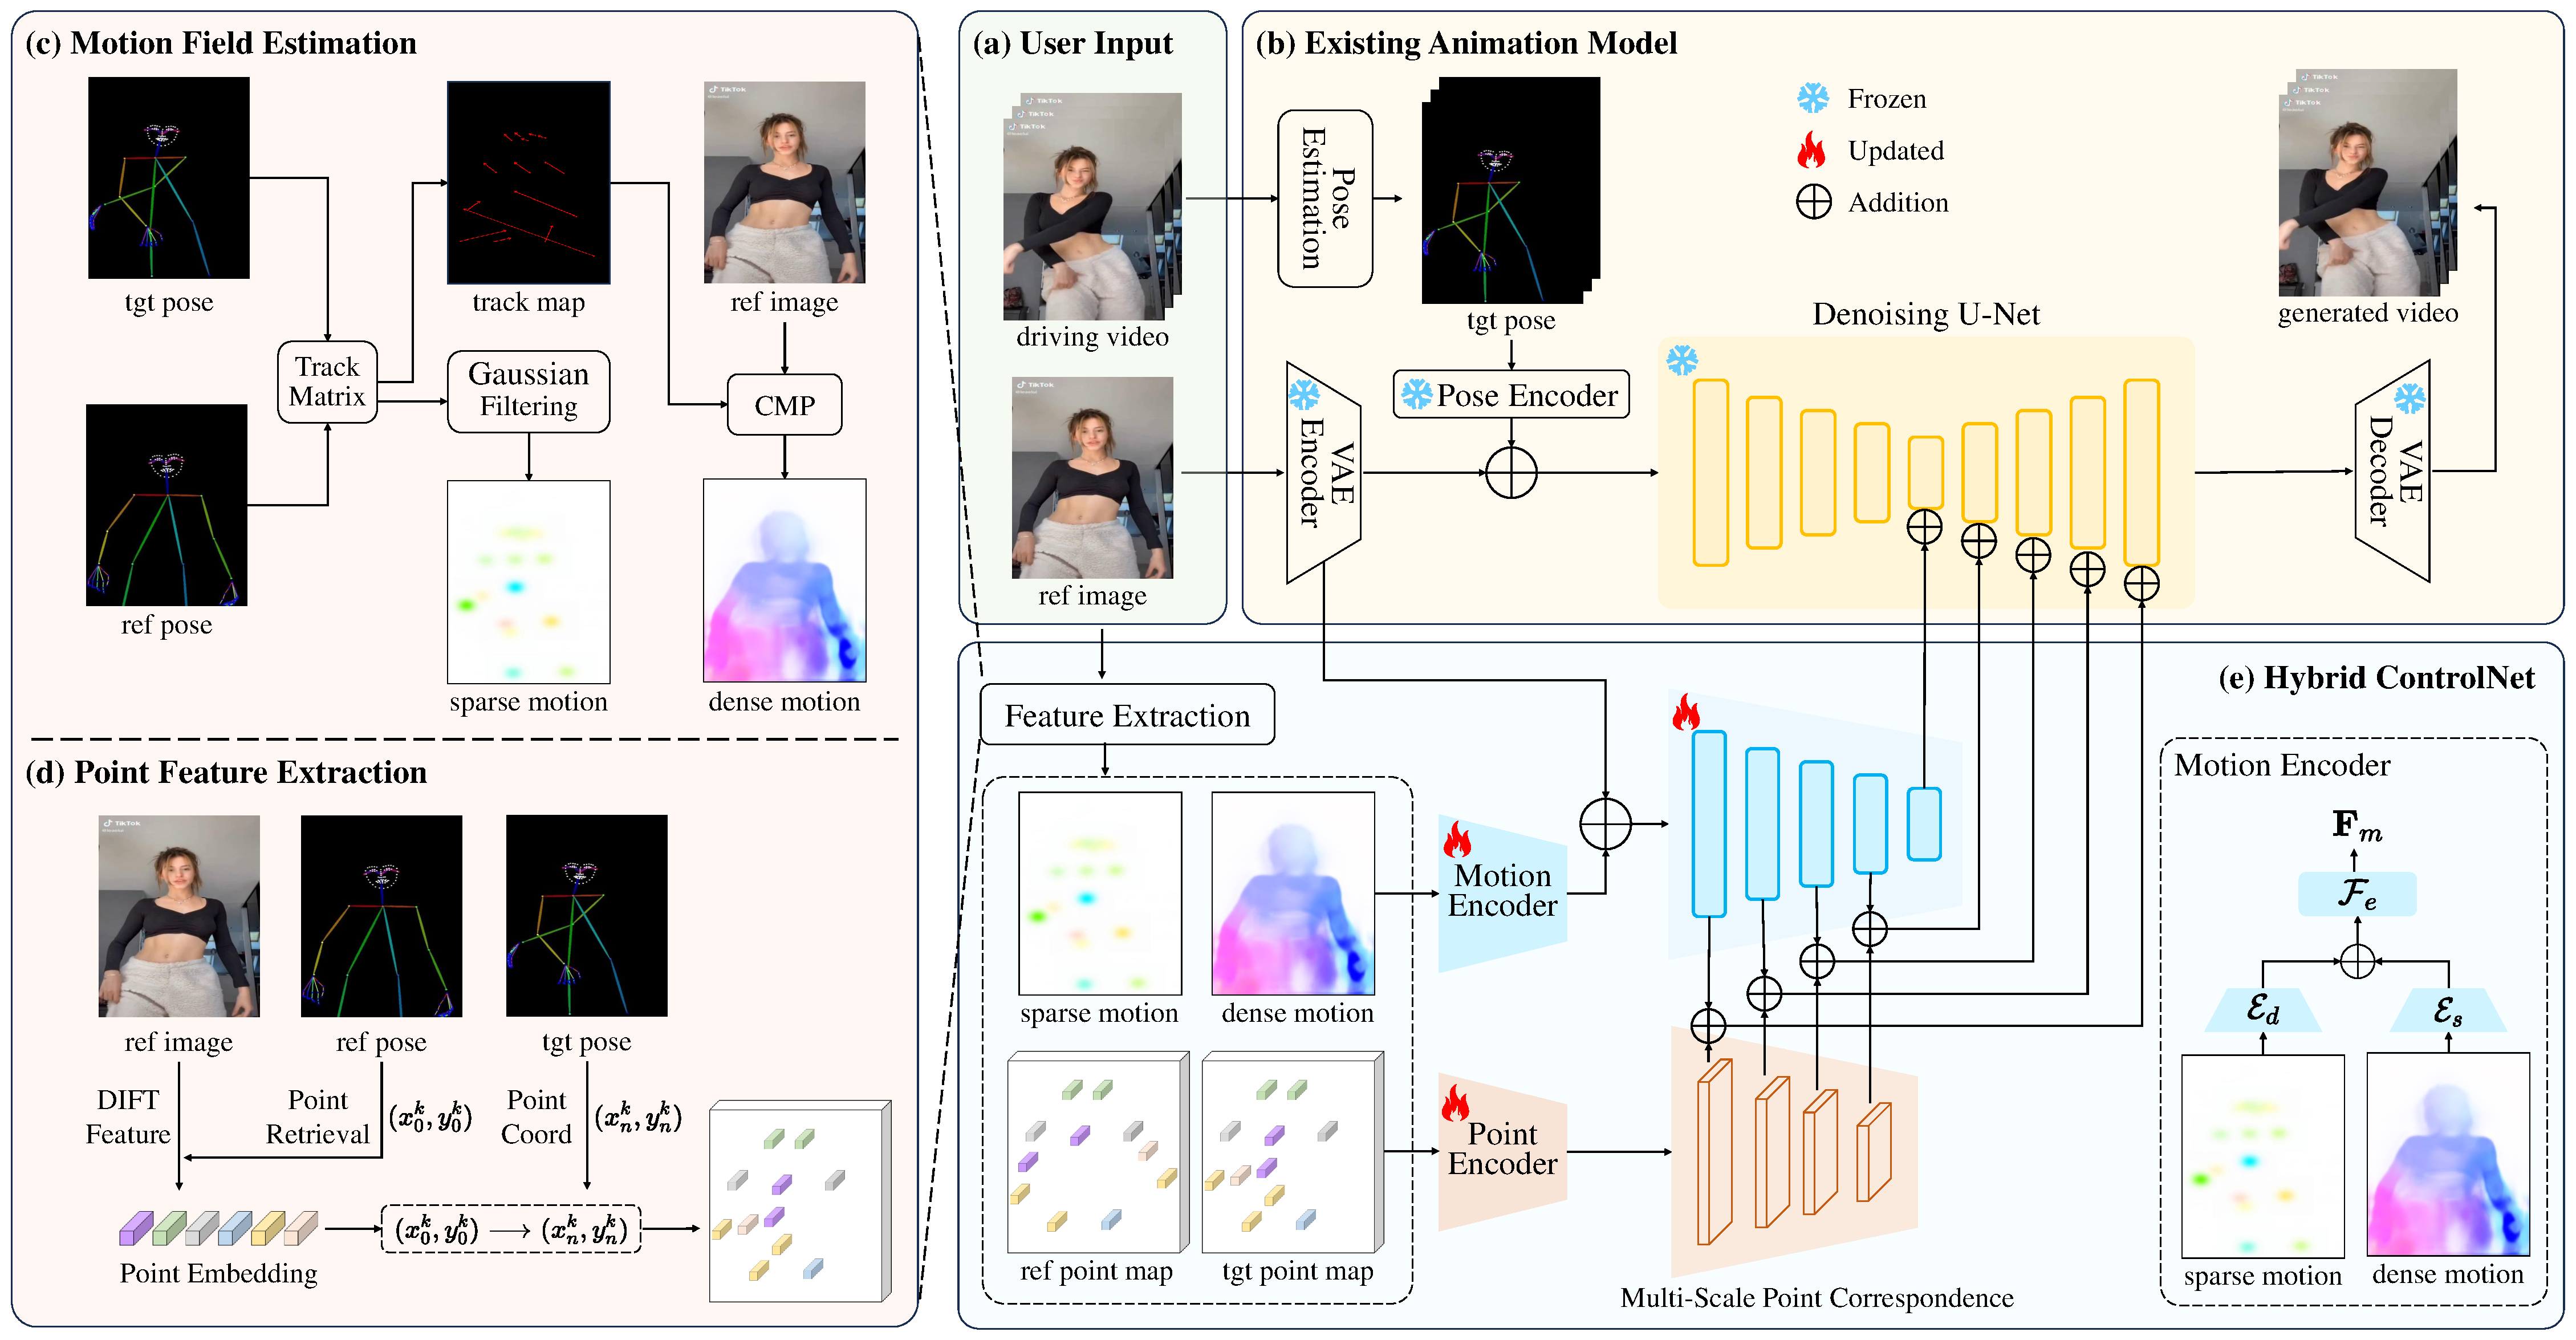
\includegraphics[width=1.0\columnwidth]{./image/pipeline.pdf}
    \vspace{-15pt}
    \caption{The overview of proposed DisPose.}
    \label{fig:pipeline}
\end{figure}
\section{DisPose}
Given a reference image $I_{\mathrm{ref}}\!\in\!\mathbb{R}^{3 \times H \times W}$ and a driving video $V\!\in\!\mathbb{R}^{N\times 3 \times H \times W}$. The core of our method is to disentangle efficient control guidance from only skeleton poses and reference images as shown in Figure~\ref{fig:pipeline}, which can be applied to existing human animation methods without additional dense inputs. We first introduce sparse and dense motion field guides in Sec.~\ref{sec: motion}. Then, we introduce reference-based keypoint correspondence in Sec.~\ref{sec: keypoint}. Finally, we introduce the pipeline of hybrid ControlNet in Sec~\ref{sec: controlnet}.
\subsection{Motion Field Guidance}
\label{sec: motion}

\textbf{Sparse Motion Field.}
We first estimate the skeleton pose by DWpose~\citep{yang2023dwpose} to obtain each frame's human key point coordinates. 
% Subsequently, the motion trajectory of all semantic points in the entire video is obtained and represented as
Subsequently, the key points of the reference image are used as starting points to track the motion displacement of all frames and represented as $P_{traj}\!=\!\{(x^k_n,y^k_n) \!\mid\! k=1\dots K, n=0\dots N\}$, where $P_{traj}$ denotes the trajectory map of the key point $k$ overall $N$ frames and $n = 0$ denotes the reference image. We calculate the track matrix $P_{s}$ as follows:
\begin{equation}
    \mathbf{P}_{s}=\{(x^k_n-x^k_{n-1}, y^k_n-y^k_{n-1}) \mid n=1\dots N\}\},
\end{equation}
% where $P_{t}$ denotes the trajectory map of the key point point $k$ over all $N$ frames, and the reference frame when $n = 0$.
where $K$ denotes the number of keypoints, $N$ denotes the number of frames, $\mathbf{P}_{s}$ denotes the trajectory map of keypoint k over all N frames, and $n = 0$ denotes the reference image.
To avoid training instability caused by overly sparse trajectory matrice, we then apply Gaussian filtering to enhance $\mathbf{P}_{s}$ to obtain the sparse motion field $\mathbf{F}_s\!\in\!\mathbb{R}^{(N-1)\times 2 \times H \times W}$ inspired by~\citep{yin2023dragnuwa, wang2024motionctrl}.

\textbf{Dense Motion Field.}
Considering that sparse control provides limited guidance and dense control is hard to obtain during inference,
% For the dense motion field, 
we transform dense guidance into the motion propagation from the reference frame to the target pose, instead of the dense signal of the target pose. Specifically, in the inference, we reconstruct the trajectory map $\mathbf{P}_{s}$ as the reference-based sparse optical flow $\mathbf{P}_{d}$ from the reference frame to each target pose as:
\begin{equation}
    \mathbf{P}_{d}=\{(x^k_n-x^k_{0}, y^k_n-y^k_{0}) \mid n=1\dots N\}\},
\end{equation}
We then predicted the reference-based dense motion filed $\mathbf{F}_d\!=\! \text{CMP}(P_{traj}, \mathbf{P}_{d}, I_{ref})\!\in\!\mathbb{R}^{(N-1)\times 2 \times H \times W}$ by condition motion propagation (CMP)~\citep{zhan2019self} based on the sparse optical flow $\mathbf{P}_{d}$ and the reference image $I_{ref}$.
CMP~\citep{zhan2019self} is a self-supervised learning-from-motion model that acquires an image and a sparse motion field and estimates the corresponding dense motion field.
Notably, the dense motion field $\mathbf{F}_d$ of each frame starts with the reference image, which avoids geometric constraints during inference.

To ensure motion estimation accuracy during training, we first extract the forward optical flow from the driving video using existing optical flow estimation models~\citep{teed2020raft, xu2023unifying}. We then use a watershed-based approach~\citep{zhan2019self} to sample the sparse optical flow $\mathbf{P}_{d}$ from the forward optical flow. See Appendix.~\ref{sec: appendix1} for details.

\textbf{Motion Encoder.} To leverage motion field as guidance, we introduce a motion encoder specifically designed for the optional flow, which includes sparse motion encoder $\mathcal{E}_s$, dense motion encoder $\mathcal{E}_d$ and feature fusion layer $\mathcal{F}_e$. $\mathcal{E}_d$ and $\mathcal{E}_s$ have the same structure and are multi-scale convolutional encoders with each stage built by \texttt{Conv-SiLU-ZeroConv}~\citep{zhang2023adding} as the basic block. The feature fusion layer $\mathcal{F}_e$ is a 2D convolution for fusing sparse motion features $\mathcal{E}_s(\mathbf{F}_s)$ and dense motion features $\mathcal{E}_d(\mathbf{F}_d)$. Finally, we compute the motion field guidance $\mathbf{F}_m$:
\begin{equation}
    \mathbf{F}_m = \mathcal{F}_e(\mathcal{E}_s(\mathbf{F}_s)+\mathcal{E}_d(\mathbf{F}_d))
\end{equation}

\subsection{Keypoint Correspondence}
\label{sec: keypoint}
\textbf{Point Feature Extraction.} 
To maintain a consistent appearance, it is crucial to correspond the content of the reference image with the motion trajectory. 
Specifically, we first extract the DIFT~\citep{tang2023emergent} features $\mathbf{D}$ of the reference image using the pre-trained image diffusion model. 

Subsequently, the keypoint embedding in the reference is obtained as $\mathbf{D}(x^k_0,y^k_0)$, where $(x^k_0,y^k_0)$ is retrieved from the reference pose.
% key point embeddings $\mathbf{D}(x^k_0,y^k_0)$ are retrieved from $\mathbf{D}$ by skeleton pose $(x^k_0, y^k_0)$.
Next, we initialize the keypoint correspondence map $\mathbf{F}_p$ with zero vectors and assign point embeddings according to the trajectory coordinates as:
\begin{equation}
\label{eq: v prob}
f^{ij}_n=\left\{\begin{array}{ll}
\mathbf{D}(x^k_0,y^k_0), & \mathrm{if} \quad i=x^k_n, j=y^k_n,  \\
0, & \mathrm{otherwise}.
\end{array}\right.
\end{equation}

Finally, we obtain the keypoint correspondence map $\mathbf{F}_p=\{f_n\!\mid\!n=1\dots N\} \!\in\!\mathbb{R}^{N\times D_p \times H \times W}$ for all frames, where $D_p$ is the feature dimension of the point embedding.

\textbf{Point Encoder.} 
To utilize the content correspondence of key points as guidance, we generate multi-scale correspondences of sparse point feature maps and make them compatible with the U-Net encoder of the {Hybrid ControlNet (Sec.4.3)}. 
% as detailed in F. 1.
We introduce the multi-scale point encoder $\mathcal{E}_p$ to maintain the key point content $\mathbf{F}_p$ from the reference image. The point encoder $\mathcal{E}_p$ consists of a series of learnable MLPs.
{
To seamlessly integrate into existing models, we extract intermediate features of the encoder of the hybrid Controlnet.
The multi-scale intermediate features of the Controlnet encoder are denoted as $\mathbf{E}^l_{enc}$, where $l$ denotes each U-Net block $l\!\in\![1, L]$.}
To match the spatial size of $\mathbf{E}^l_{enc}$, we apply downsampling to the feature map between the encoder layers. We compute the multi-scale keypoint correspondence as follows:
\begin{equation}
    \mathbf{F}_c^l = \mathcal{E}_p^l(\phi(\mathbf{F}_p, H^l, W^l)),
\end{equation}
where $(H^l, W^l)$ are denote the spatial dimension of the $l$-th U-Net block and $\phi$ means downsampling operation. Therefore, $\mathbf{F}_c^l$ shares the same size as $\mathbf{E}^l_{enc}$.
Finally, $\mathbf{F}_c$ are added elementwisely to the intermediate feature $\mathbf{E}^l_{enc}$ of the U-Net encoder as guidance: $\mathbf{E}^l_{enc}\!=\!\mathbf{E}^l_{enc}+\mathbf{F}_c^l$.


\subsection{Plug-and-play Hybrid ControlNet}
\label{sec: controlnet}
After obtaining motion field guidance and keypoint correspondence, we aim to integrate these control guidance seamlessly into the U-Net architecture of existing animation models.
Inspired by ControlNet~\citep{zhang2023adding}, We design a hybrid ControlNet $\mathcal{F}$ to provide additional control signals for the existing animation model as shown in Figure~\ref{fig:pipeline}(e).
% Specifically, we consider freeze denoising U-Net and pose encoder. 
Specifically, given an animation diffusion model based on the U-Net architecture, we freeze all its modules while allowing the motion encoder, point encoder and hybrid ControlNet to be updated during training. 
Subsequently, $\mathbf{F}_m$ is added to the noise latent before being input into the hybrid ControlNet. Considering the high sparsity of the point feature $\mathbf{F}_c$, we correspondingly add $\mathbf{F}_c$ to the input of the convolutional layer. Notably, the U-Net encoder intermediate feature $\mathbf{E}_{enc}$ in Sec.~\ref{sec: keypoint} is from hybrid ControlNet rather than denoising U-Net. Finally, 
the control condition is computed as:
\begin{equation}
    \boldsymbol{r}=\mathcal{F}(\boldsymbol{z}_{{t}} \mid \mathbf{F}_m, \mathbf{F}_c, {t})
\end{equation}
where $\boldsymbol{r}$ is a set of condition residuals added to the residuals for the middle and upsampling blocks in the denoising U-Net.
\begin{figure}[t]
  \centering
  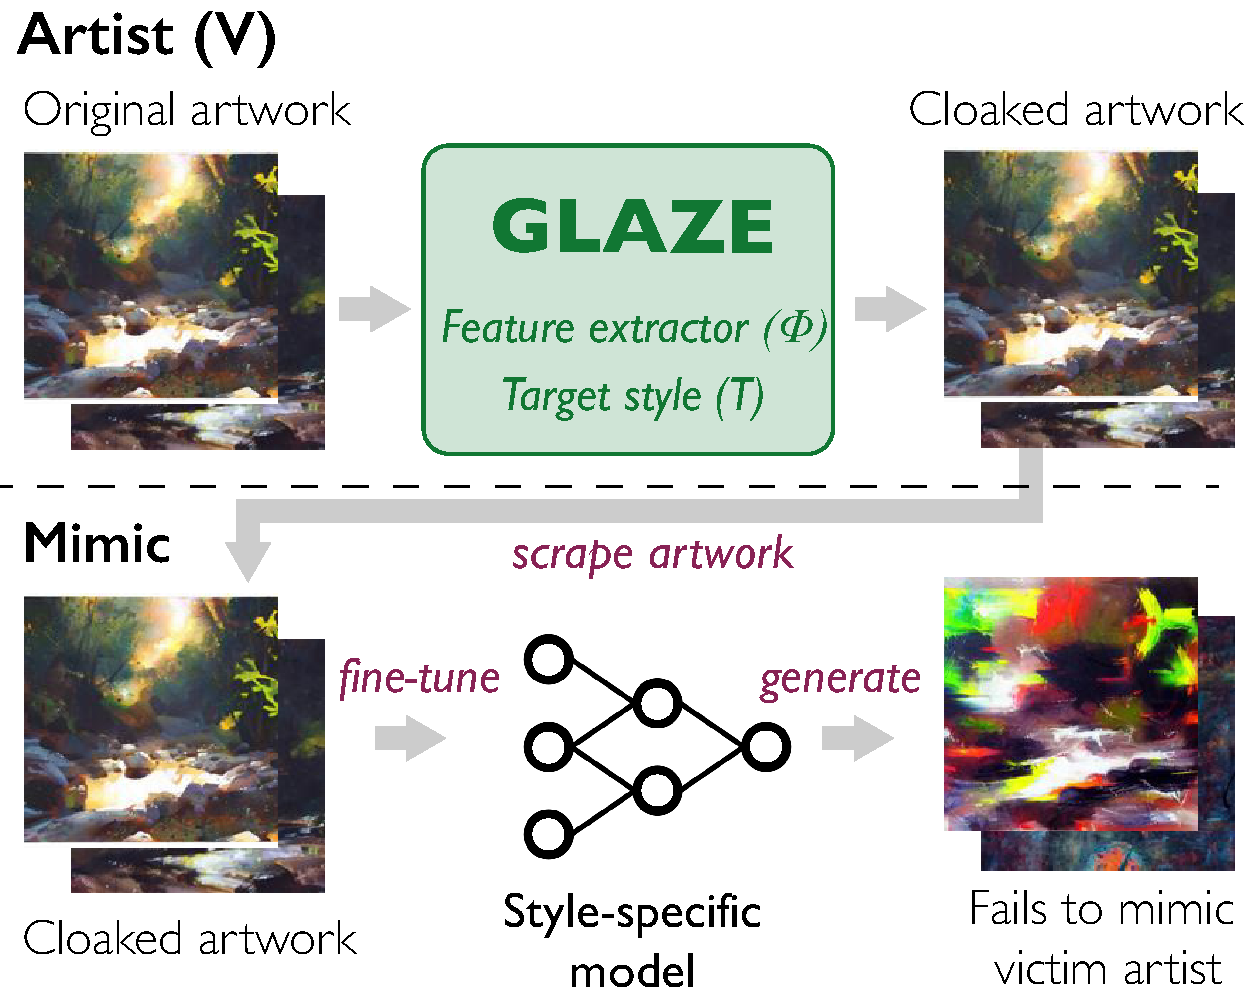
\includegraphics[width=0.9\columnwidth]{plots/overview/cloak-scenario-emily.pdf}
  \caption{Overview of \system{}, a system that protects victim artists from AI style mimicry by cloaking their online artwork. ({\bf Top}) An artist $V$ applies the cloaking algorithm (uses a feature extractor $\Phi$ and a target style $T$) to generate cloaked versions of $V$'s art pieces. Each cloak is a small perturbation unnoticeable to human eye. ({\bf Bottom}) A mimic scrapes the cloaked art pieces from online and uses them to fine-tune a model to mimic $V$'s style. When prompted to generate artwork in the style of $V$, mimic's model will generate artwork in the target style $T$, rather than $V$'s true style. }
  \label{fig:cloaking}
\end{figure}

\begin{figure}[t]
  \centering
  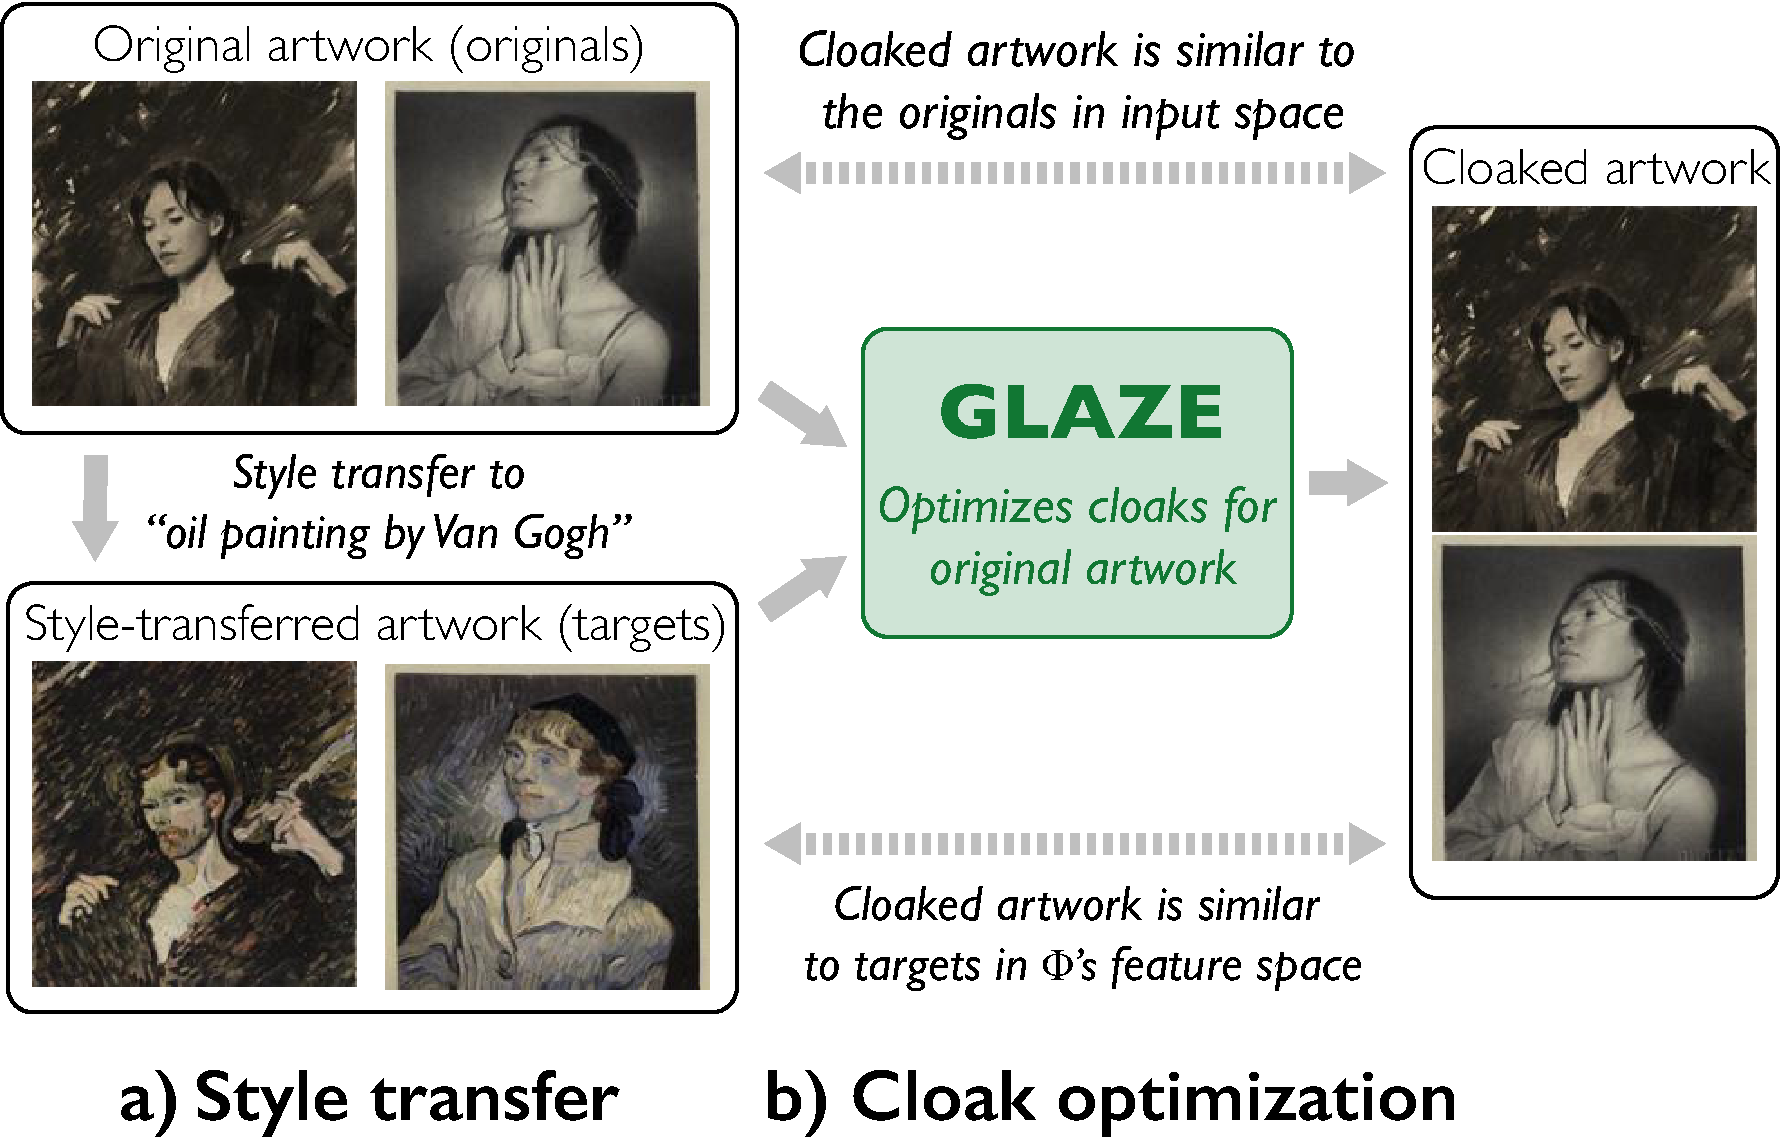
\includegraphics[width=1\columnwidth]{plots/overview/cloak-intuition-2-emily.pdf}
  \caption{High level overview of how \system{} perturbs the style-specific features of the artwork. {\bf a)} \system{} style transfers the original artwork to a different style, which changes its style but leaves other features unaltered. {\bf b)} \system{} optimizes a cloak that makes the artwork's features representation match that of the style-transferred art, while constraining the amount of visible changes to the artwork.  }
  \label{fig:cloak-intuition}
  \vspace{-0.3cm}
\end{figure}

\begin{figure}[t]
  \centering
  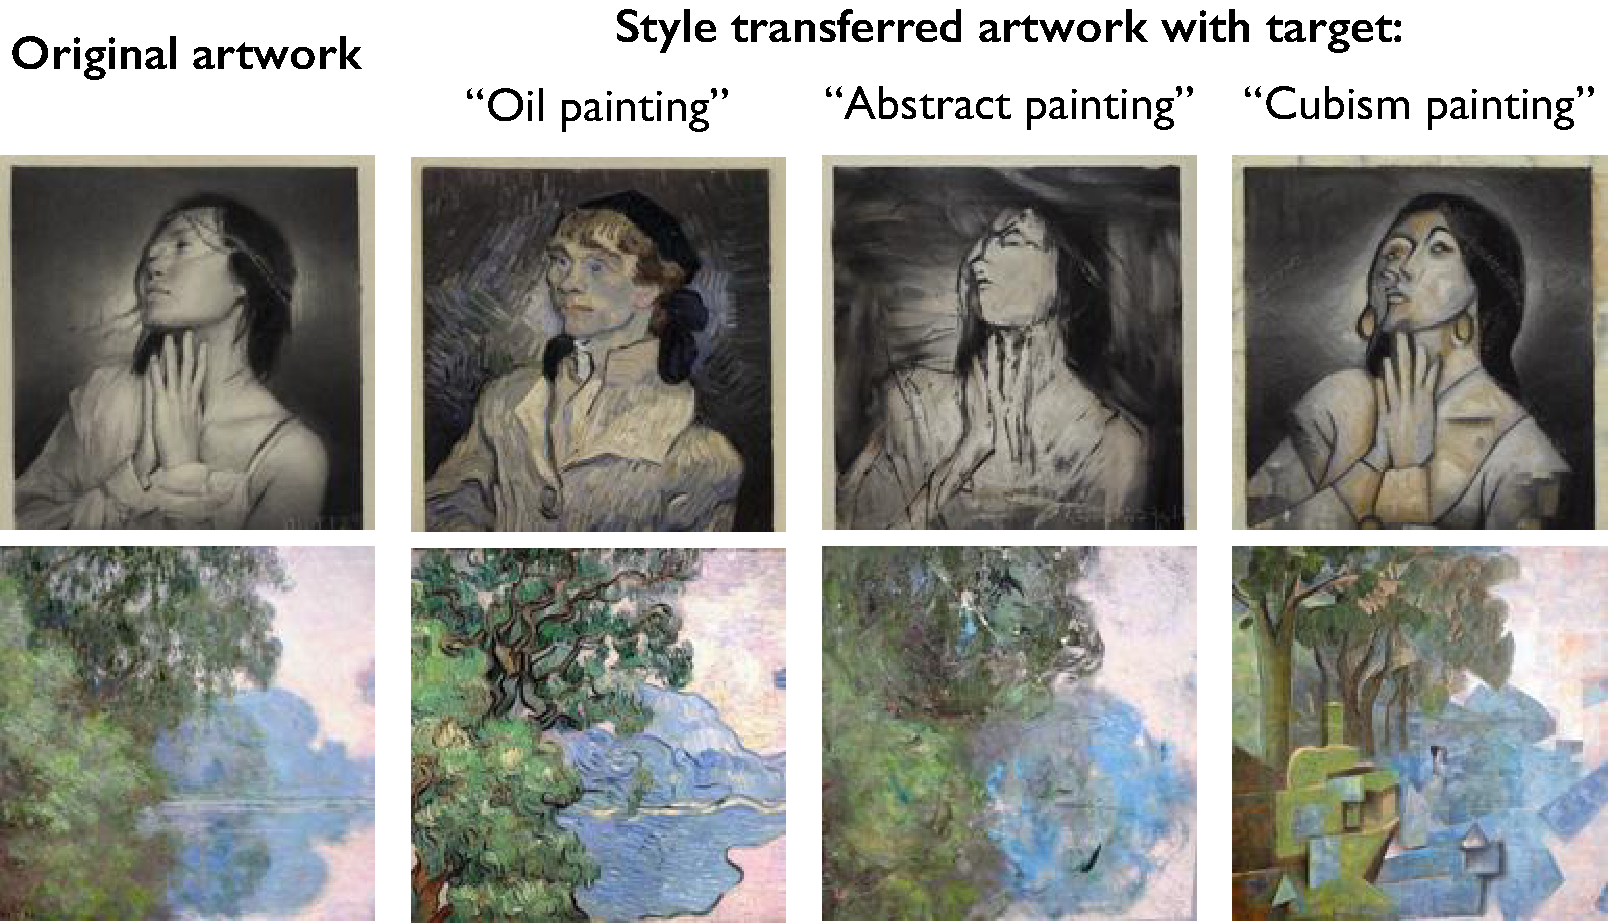
\includegraphics[width=1\columnwidth]{plots/eval/style-transfer-example.pdf}
  \caption{Example style-transferred artwork with different target styles. }
  \label{fig:transfer-examples}
\end{figure}

\secspace
\section{Disrupting Style Mimicry with Glaze} 
\label{sec:design}

In this section, we introduce \system{}, its design intuition followed by the
detailed algorithm. 

\secspace
\subsection{Design Intuition}
\label{sec:intuition-cloak}

Our key intuition is to identify and isolate \textit{style-specific features}
of an artist's original artwork, \ie the set of image features that
correspond to artistic style. Then \system{} computes cloaks while focusing
the perturbation budget on these style-specific features to maximize impact
on stylistic features.

As discussed, identifying and calculating style-specific features in model's
feature space is difficult due to the poor interpretability of model features
and how art style manifests differently across artworks. We overcome these two
challenges by designing a style-dependent and artwork-dependent method that
operates at image space. Given an artwork, we leverage ``style transfer,'' an
end-to-end computer vision technique, to modify and isolate its style
components. ``Style transfer'' transforms an image into a new image with a
different style (\eg from impressionist style to cubist style) while keeping
other aspects of the image similar (\eg subject matter and location).
% This is ideal for our use case, where protection must focus
% on style-specific features.

We leverage style transfer in our protection technique as follows. Given an
original artwork from the victim artist, we apply style-transfer to produce a
similar piece of art with a different style, \eg in style of ``an oil
painting by Van Gogh'' (Figure~\ref{fig:cloak-intuition} a). The new
version has similar content to the original, but its style mirrors that
of Van Gogh. We show more style-transfer examples with different target styles in
Figure~\ref{fig:transfer-examples}. Now, we can use the style-transferred
artwork as projection target to guide the perturbation computation. This
perturbs the original artwork's style-specific features towards that of
the style-transferred version. We do this by optimizing a cloak that, when
added to the original artwork, makes its feature representation similar to
the style-transferred image. Since the content is identical between the pair
of images, cloak optimization will focus its perturbation budget on style
features. 

\secspace
\subsection{Computing Style Cloaks} 

Using this approach, we compute style cloaks to disrupt style mimicry as
follows. Given an artwork ($x$), we use an existing feature extractor to
compute the style-transferred version of $x$ into target style $T$: $\Omega(x, T)$.
%style-transfer neural network that style transfers image $x$ and outputs
We then compute a style cloak $\delta_x$, such that $\delta_x$ moves $x$'s
style-specific feature representation to match that of $\Omega(x, T)$ while
minimizing visual impact. The cloak generation optimization is:

\secspace
\begin{eqnarray}
   &\min\limits_{\delta_x} Dist\left( \Phi(x + \delta_x), \Phi (\Omega(x, T))\right),  \label{eq:cloakopt}\\
  & \text{subject to } \; |\delta_x|< p, \nonumber
\end{eqnarray} 

\noindent where $\Phi$ is a generic image feature extractor commonly used in
text-to-image generation tasks, $Dist(.)$ computes the distance of two
feature representations, $|\delta_x|$ measures the perceptual perturbation
caused by cloaking, and $p$ is the perceptual perturbation budget. 

As discussed in \S\ref{sec:intuition-cloak}, the use of the style-transferred
image $\Omega(x, T)$ guides the cloak optimization in Eq~(\ref{eq:cloakopt})
to focus on changing style-specific image features. To maximize cloak
efficacy, the target style $T$ should be dissimilar from artist's original
style in the feature space. We discuss our heuristic for selecting target styles in
\S\ref{sec:design}.

\secspace
\subsection{Detailed System Design}
\label{sec:design-details}

Now we present the detailed design of \system{}. Given a victim
artist $V$, \system{} takes as input the set of $V$'s artwork to be shared
online $X_V$, an image feature extractor $\Phi$, a style-transfer model
$\Omega$, and perturbation budget $p$. Note that in many cases, a single
model (e.g. Stable Diffusion) provides both $\Phi$ and $\Omega$.

\para{Step 1: Choose Target Style.}  The selected target style $T$
should be sufficiently different from $V$'s style in model feature space to
maximize chances of disrupting style mimicry. For example, Fauvism and
Impressionism are distinct art styles that often look visually similar to the
untrained eye. Image of an impressionist painting style cloaked to Fauvism
might not produce a visually discernible effect on model-generated
paintings. Note that an artist can maximize their ability to avoid mimicry if
they consistently style cloak all their artwork towards the same target $T$.

For a new user, \system{} uses the following algorithm to randomly select $T$ from a set
of candidate styles reasonably different from $V$'s style. The algorithm
first inspects a public dataset of artists, each with a specific style (\eg
Monet, Van Gogh, Picasso). For each candidate target artist/style, it selects
a few images in that style and calculates their feature space centroid using
$\Phi$. It also computes $V$'s centroid in $\Phi$ using $V$'s artwork. Then,
it locates the set of candidate styles whose centroid distance to $V$'s
centroid is between the $50$ to $75$ percentile of all candidates. Finally,
it randomly selects $T$ from the candidate set.

\para{Step 2: Style transfer. } \system{} then leverages a pre-trained
style-transfer model $\Omega$~\cite{rombach2022high} to generate the
style-transferred artwork for optimization. Given each art piece $x \in
X_V$ and target style $T$, it style transfers $x$ to target style $T$ to
produce style-transferred image $\Omega(x, T)$.  

\para{Step 3: Compute cloak perturbation.} Then, \system{} computes the
cloak perturbation, $\delta_x$ for $x$, following the optimization defined
by eq. (\ref{eq:cloakopt}), subject to $|\delta_x| < p$. Our implementation
uses LPIPS (Learned Perceptual Image Patch
Similarity)~\cite{zhang2018unreasonable} to bound the perturbation. Different
from the $L_p$ distance used in previous
work~\cite{carlini2017towards,kurakin2016adversarial,sabour2015adversarial},
LPIPS has gained popularity as a measure of user-perceived image
distortion~\cite{cherepanova2021lowkey,laidlaw2020perceptual,rony2021augmented}. Bounding
cloak generation with this metric ensures that cloaked versions of images are
visually similar to the originals. We apply the \textit{penalty
  method}~\cite{nocedal2006numerical} to solve the optimization in
eq.(\ref{eq:cloakopt}) as follows:  

\vspace{-0.05in}
\begin{equation} \label{eq:optdetail} \vspace{-0.03in} 
 \underset{\delta_x}{\text{min }}||\Phi(\Omega(x, T)), \Phi(x + \delta_x) ||_2^2 + \alpha \cdot max(LPIPS(\delta_x)-p, 0) 
\end{equation}

\noindent where $\alpha$ controls the impact of the input perturbation. $L_2$
distance is used to calculate feature space distance.

\para{Upload artwork online.} Finally, the artist posts the cloaked artwork
online. For artists already with a large online presence, they can cloak and
re-upload artwork on their online portfolio.
While updating online images is not always possible, 
\system{} can be effective even when the mimic's model has significant amount
of uncloaked art (\S\ref{sec:robust-eval}).

\secspace
\subsection{On the Efficacy of Style Cloaks}
\label{sec:cloak-effect}

\system's style cloaks work by shifting feature representation of artwork in
the generator model. But how much shift do we need in order to have a
noticeable impact on mimicked art?


Two reasons suggest that even small shifts in style will have a meaningful
impact in disrupting style mimicry. First, generative models used for style
mimicry have {\em continuous} output spaces, \ie any shift in image feature
representation results in changes in the generated image.  Because generative
models are trained to interpolate their continuous feature
spaces~\cite{white2016sampling,upchurch2017deep}, any shift in the model's
representation of art style results in a new style, a ``blend'' between the
artist and the chosen target style.  
% the cloaked image with an \textbf{in-between style}, \ie a blended style of
% the original and target style,
Second, mimicked artwork must achieve reasonable quality and similarity in
style to the artist to be useful. Small shifts in the style space often
produce incoherent blends of conflicting styles that are enough to disrupt
style mimicry, \eg thick oil brushstrokes of Van Gogh's style mixed into a realism portrait.

These two factors contribute to \system{}'s success in more challenging
scenarios (\S\ref{sec:robust-eval}), and its robustness against
countermeasures (e.g. adversarial training) that succeed against cloaking
tools for facial recognition (\S\ref{sec:counter}).


\section{Evaluation}
\label{sec:eval-cloak}

In this section, we evaluate \system's efficacy in protecting artists from
style mimicry. We first describe the datasets, models, and experimental
configurations used in our tests. Then we present the results of \system's
protection in a variety of settings. Due to \system's highly visual nature,
we evaluate its performance using both direct visual assessment by
\textbf{human artists} in a user study, and \textbf{automated metrics} (see
\S\ref{sec:metrics} for details).

\para{Summary of results.} Over $93\%$ of artists surveyed believe \system{}
effectively protects artists' styles from AI style mimicry
attacks. Protection efficacy remains high in challenging settings, like when
the mimic has access to unprotected artwork. \system{} also achieves high
protection performance against a real-world mimicry-as-a-service platform. Of
our $1156$ artist participants, over $92\%$ found the perturbations
introduced by cloaking small enough not to disrupt the value of their art,
and over $88\%$ would like to use \system{} to protect their own artwork from
mimicry attacks.

\secspace
\subsection{Experiment Setup}
\label{sec:cloak-setup}

\para{Mimicry dataset. } We evaluate \system's performance in protecting the styles of the following two groups of artists: 

\vspace{-0.2cm}
\begin{packed_itemize}
\item {\em Current artists}: $4$ professional artists let us use their
  artwork in our experiments. These artists have different styles and
  backgrounds (\eg full-time/freelancers, watercolor painters/digital
  artists, well-known/independent). Each provided us with between $26$ to
  $34$ \textit{private} original art pieces for our experiments. We use
  perceptual hashing~\cite{ke2004efficient} to verify that none of these are
  included in existing public datasets used to train generic text-to-image
  models (e.g.~\cite{schuhmann2022laion,changpinyo2021conceptual}).  

\item {\em Historical artists}: We also evaluate \system{}'s protection on
  $195$ historical artists (\eg van Gogh, Monet) from the WikiArt
  dataset~\cite{saleh2015large}. The WikiArt dataset contains 42,129 art
  pieces from $195$ artists. Each art piece is labeled with its genre (\eg
  impressionism, cubism). We randomly sampled $30$ art pieces from each
  artist to use in style mimicry attacks. Generic text-to-image models found
  online have been trained on some artwork from these artists. Using this art
  simulates a more challenging scenario in which a famous artist attempts
  to disrupt a model that already understands their style.
\end{packed_itemize}
\vspace{-0.2cm}

\para{Mimicry attack setup. } We recreate the strongest-possible mimicry
attack scenario, based on techniques used in real-world mimicry
incidents~\cite{ruiz2022dreambooth,sam-steal,hollie-steal},
that works as follows. First, we take art pieces from the victim artist $V$
and generate a text caption for each piece using an image captioning
model~\cite{luo2022vc}. \revise{The pretrained image captioning model generates a short 
sentence to describe the image. We found that this model can correctly caption protected images (examples in Figure~\ref{fig:data-examples}), likely because \system{} focuses on perturbing style features while the captioning models focus on image content.} Then, we append the artist's name to each caption,
\eg ``mountain range \textit{by Vincent van Gogh}''. Finally, we fine-tune a pre-trained generic text-to-image model
(details below) on the caption/image pairs. 

We use $80\%$ of the art pieces from the victim artists to fine-tune models
that mimic each artist's style, reserving the rest for testing. We fine-tune
for $3000$ optimization steps, which we find achieves the best mimicry
performance (Figure~\ref{fig:success-iter} in Appendix). We then use the
fine-tuned, style-specific model to generate mimicked artwork in style of
each victim artist. We query the model using the generated captions (which
include $V$'s name) from the held-out test artwork set. We generate $5$
pieces of mimicked art for each text caption using different random seeds and
compare these to the real victim art pieces with this caption. Additional
details on training and generation parameters, as well as its sensitivity to
random seed selection and the number of training art pieces are in Appendix~\ref{app:mimicry}.  

% Fine-tuning a style-specific mimicry model takes 56.4 minutes on average on one Titan RTX GPU~\footnote{This takes longer than real-world mimicry incidents because we finetune more steps for better mimicry performance.}. 

\para{Text-to-image models.} We use two state-of-the-art, public, generic text-to-image models in our experiments: 

\vspace{-0.2cm}
\begin{packed_itemize}
\item \textit{Stable Diffusion (SD)}: Stable Diffusion is a popular and
  high-performing open-source text-to-image model~\cite{stable2-1},trained
  on 11.5 million images from the LAION dataset~\cite{schuhmann2022laion}. SD
  training takes over 277 GPU months (on A100 GPU) and costs around
  \$600K~\cite{stable2-1}. SD uses diffusion methods to generate images and
  achieves state-of-the-art performance on several
  benchmarks~\cite{rombach2022high}. Viewed as one of the best open-source
  models, SD has powered many recent developments in text-to-image
  generation~\cite{blender-plugin,novelai-update,gimp,aigame}. We
  use SD version 2.1 in the paper~\cite{stable2-1}, the most up-to-date
  version as of December 2022.  

\item \textit{DALL$\cdot$E-mega (\dalleM)}: \dalleM-mega, an updated version
  of the more well-known \dalleM-mini, is an open-source model based on
  OpenAI's \dalleM~1~\cite{ramesh2021zero}. The model leverages a VAE for
  image generation and is trained on 17 million images from three different
  datasets~\cite{sharma-etal-2018-conceptual,changpinyo2021conceptual,thomee2016yfcc100m}. Training
  takes 2 months on 256 TPUs~\cite{mini-training}. While \dalleM~ performs
  worse than diffusion-based models like SD, we use it to evaluate how
  \system~generalizes to different model architectures.  
\end{packed_itemize}

\vspace{-0.2cm}

\para{\system~configuration. } We generate cloaks for each of victim $V$'s
art pieces following the methodology of \S\ref{sec:design-details}. First, we
use the target selection algorithm to select a target style $T$. We choose
from a set of $1119$ candidate target styles, collected by querying the
WikiArt dataset with artist and genre names, \eg ``Impressionism painting by
Monet''~\footnote{One artist may paint in multiple styles, resulting in
  multiple candidate target styles from a single artist.}. We then style
transfer each victim art piece into the target style leveraging the style
transfer functionality of stable diffusion model (stable diffusion model has
both text-to-image and style transfer functionality). \revise{A style transfer model takes
in an original image and a target prompt as input. Leveraging a similar diffusion process, the model
modifies the original image to a style similar to that described in the target prompt. More information on style transfer can be found in ~\cite{saharia2022palette}}. Finally, we optimize a cloak for each art piece
using Eq.~\ref{eq:optdetail} by running the Adam optimizer for $500$
steps. \revise{We benchmark \system{}'s runtime on artwork with resolution ranging 
from $512$ to $6000$ pixels, using SD's feature extractor (ViT model with 83 million parameters). } It takes an average of $1.2$ mins on Titan RTX GPU and $7.3$ mins on a
single Intel i7 CPU to generate a cloak for a single piece of art. 

In our initial experiments, we assume \system{} generates cloaks using the
same image feature extractor as the mimic (e.g. SD's or \dalleM's feature
extractor). We relax this assumption and evaluate
\system{}'s performance when artists and mimics use different feature
extractors in \S\ref{sec:robust-eval}.

\secspace
\subsection{Evaluation Metrics} 
\label{sec:metrics}

We evaluate our protection performance using both visual assessment and feedback from
human artists, and a scalable metric. Here, we describe the setup of our
evaluation study and define the exact metrics used for evaluation.  

% \vspace{-0.2cm}
% \begin{packed_itemize}
\para{Artist-rated protection success rate (Artist-rated PSR): } The user
studies ask artists to rate the performance of \system. We generate a dataset
of mimicry attacks on $13$ victim artists (the $4$ current artists and $9$
randomly chosen historical artists) across $23$ protection scenarios
(including ones in \S\ref{sec:counter}). For each participant, we randomly
select a set of mimicry attacks out of these $13 \times 23$ settings and ask
them to evaluate protection success.  For each mimicry attempt, we show
participants $4$ mimicked art pieces and $4$ original art pieces from the
victim artist. \revise{Using original art pieces as an indicator of the human
artist's style,} we ask participants to consider the mimicked art, and rate the success of 
\system{}'s
protection on a 5-level Likert scale (ranging from ``not successful at all''
to ``very successful''). Each mimicry attempt is evaluated by at least $10$
participants. We define \textit{artist-rated PSR} as the percent of
participants who rated \system{}'s protection as ``successful'' or ``very
successful.''  Our user studies primarily focus on artists, as they would be
most affected by this technology. We found though, that not all current
artists despise AI art, and some view it as a new avenue for a different form
of artistry.

\para{CLIP-based genre shift: } We define a new metric based on
CLIP~\cite{radford2021learning}, using the intuition that \system{} succeeds
if the mimicked art has been impacted enough by \system{} to be classified
into a \textit{different art genre} from the artist's original artwork. We
leverage CLIP model's ability to classify art images into art genres. Given a
set of mimicked art targeting an artist $V$, we define \textit{CLIP-based
  genre shift rate} as the percentage of mimicked art whose top 3 predicted
genres do not contain $V$'s original genre. A higher genre shift rate means
more mimicked art belongs to a different genre from the victim artist, and thus
means more successful protection.

To calculate the genre shift we use a set of $27$ historical genres from
WikiArt dataset and $13$ digital art genres~\cite{digital-styles} as the
candidate output labels. In Appendix~\ref{app:clip}, we show that a
pre-trained CLIP model is able to achieve high genre classification
performance. We report the average CLIP-based genre shift for all 199 victim
artists across all mimicked artworks.

We use CLIP-based genre shift as a supplemental metric to evaluate \system{}
because it is only able to detect style changes at the granularity of art
genres.
% checks whether the mimicked artwork belongs to a different
% art genre as artist's true genre.
However, mimicry attacks also fail when
\system{} causes the mimicked artwork quality to be very low, something that 
CLIP cannot measure. Measuring the quality of generated image has been a
challenging and ongoing research problem in computer
vision~\cite{kynkaanniemi2022role,blau2018perception,karras2020training}.


\begin{figure*}[t]
  \centering
  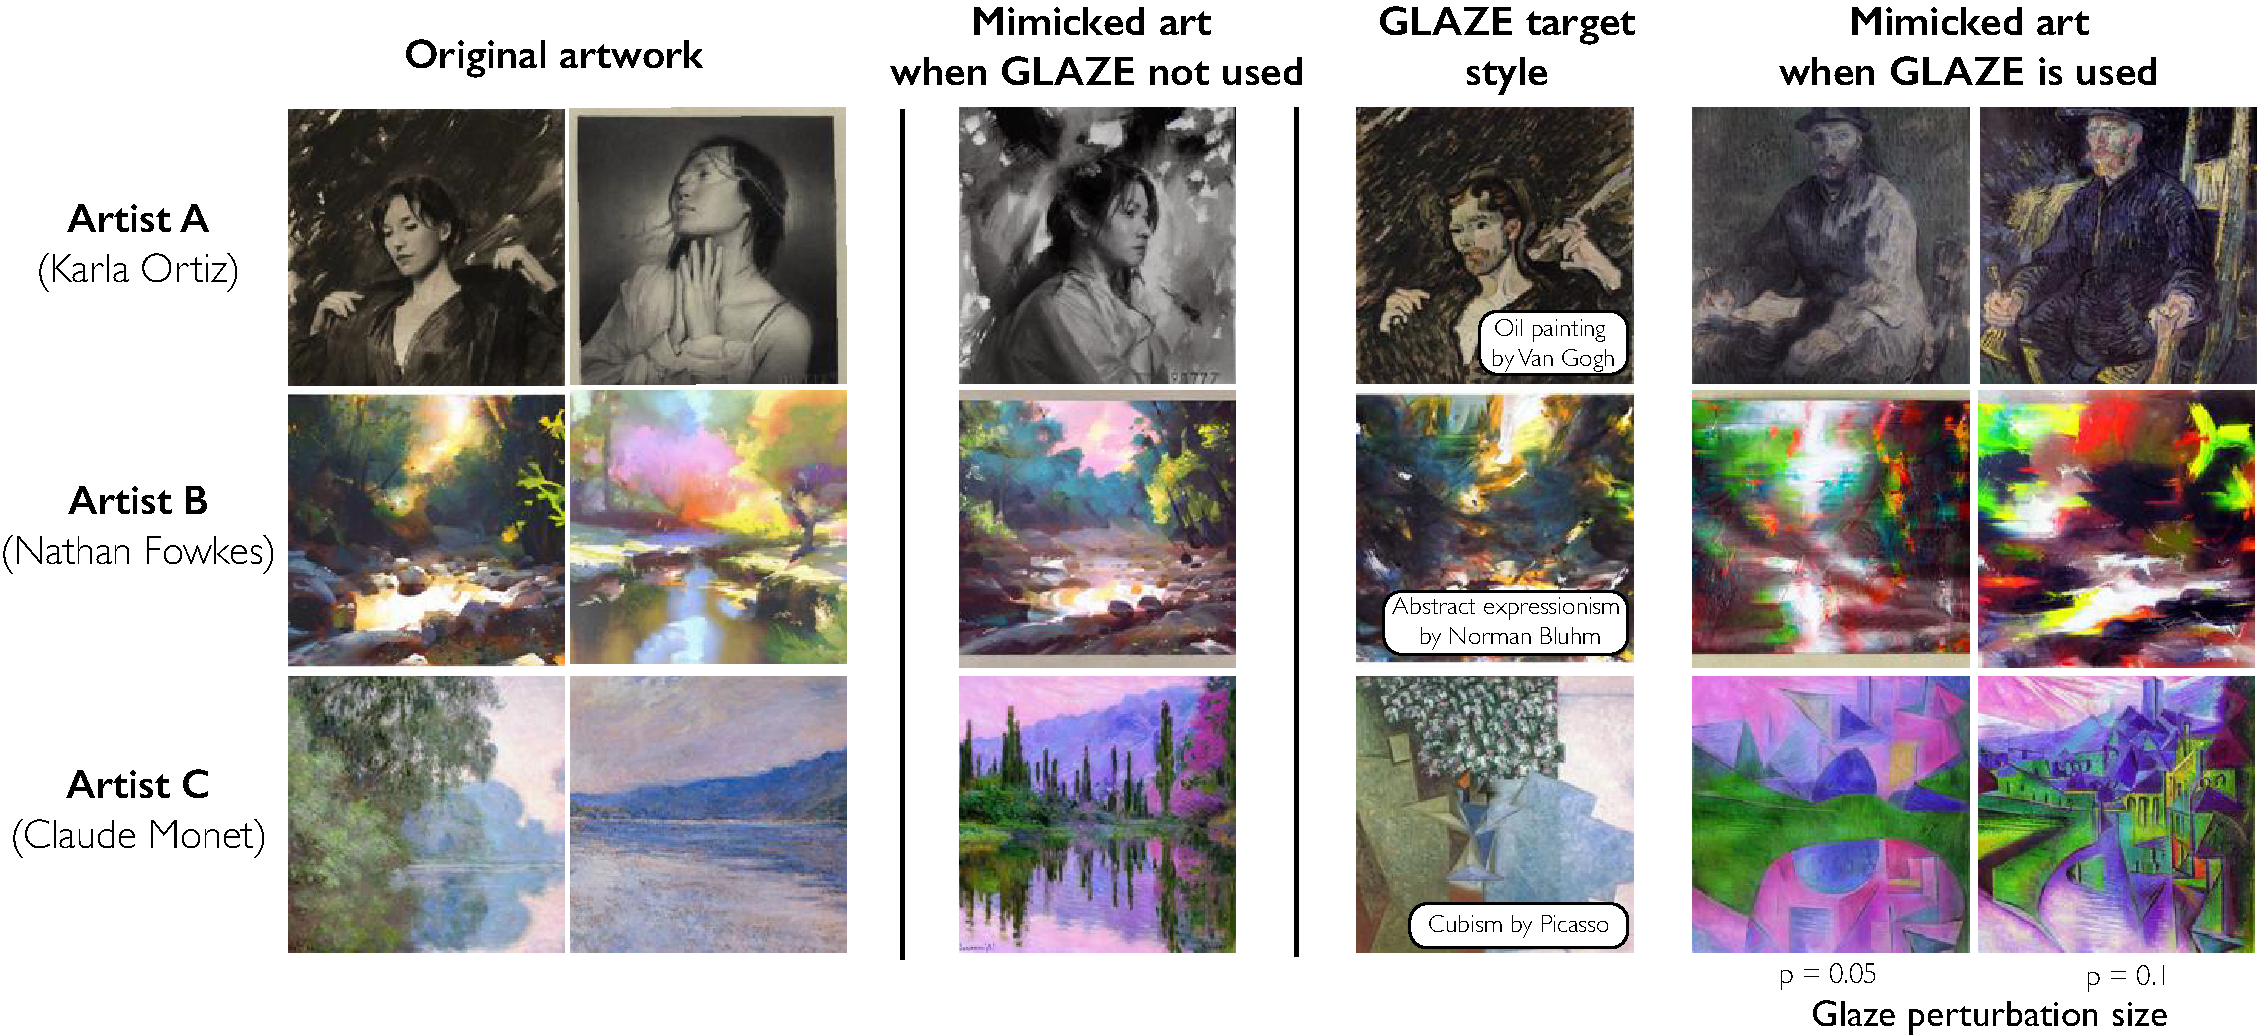
\includegraphics[width=0.9\linewidth]{plots/eval/big-result-full-emily.pdf}
  \vspace{-0.1in}
  \caption{Example \system{} protection results for three artists. {\bf
      Columns 1-2}: artist's original artwork; {\bf column 3}: mimicked
    artwork when artist does not use protection; {\bf column 4}:
    style-transferred artwork (original artwork in column 1 is the source)
    used for cloak optimization and the name of target style; {\bf column
      5-6}: mimicked artwork when artist uses cloaking protection with
    perturbation budget $p=0.05$ or $p=0.1$ respectively. All mimicry
    examples here use SD-based models.
  } %The images can be zoomed for a closer look when viewing the paper digitally. )}
  \label{fig:core-res}
\end{figure*}

\begin{table}[t]
  \centering
  \resizebox{0.5\textwidth}{!}{
  \centering
\begin{tabular}{cccccc}
\toprule
\multirow{2}{*}{\textbf{\begin{tabular}[c]{@{}c@{}} \\ Generic \\ model\end{tabular}}} & \multirow{2}{*}{\textbf{\begin{tabular}[c]{@{}c@{}}\\ Artist \\ dataset\end{tabular}}} & \multicolumn{2}{c}{\textbf{w/o \system{}}} & \multicolumn{2}{c}{\textbf{w/ \system{} (p=0.05)}} \\ \cmidrule{3-6} 
 &  & \begin{tabular}[c]{@{}c@{}}Artist-rated \\ PSR\end{tabular} & \begin{tabular}[c]{@{}c@{}}CLIP-based \\ genre shift\end{tabular} & \begin{tabular}[c]{@{}c@{}}Artist-rated \\ PSR\end{tabular} & \begin{tabular}[c]{@{}c@{}}CLIP-based \\ genre shift\end{tabular} \\ \midrule
\multirow{2}{*}{SD} & Current & $4.6 \pm 0.3\%$ & $2.4 \pm 0.2\%$ & $94.3 \pm 0.8\%$ & $96.4 + 0.5\%$ \\
 & Historical & $4.2 \pm 0.2\%$ & $1.3 \pm 0.2\%$ & $93.3 + 0.6\%$ & $96.0 + 0.3\%$ \\ \midrule
\multirow{2}{*}{\dalleM~} & Current & $31.9 \pm 3.5\%$ & $6.4 \pm 0.8\%$ & $97.4 \pm 0.2\%$ & $97.4 + 0.3\%$ \\
 & Historical & $29.8 \pm 2.4\%$ & $5.8 \pm 0.6\%$ & $96.8 \pm 0.3\%$ & $97.1 + 0.2\%$ \\ \bottomrule
\end{tabular}
  }
  \vspace{-0.1in}
  \caption{\system{} has a high protection success rate, as measured by
    artists and CLIP, against style mimicry attacks. We compare protection
    success when artists do not use \system{} vs. when they do (with
    perturbation budget 0.05). }
  \label{tab:psr-core-table}
  \vspace{-0.3cm}
\end{table}

\begin{figure*}[t]
  \centering
  \begin{minipage}{0.32\textwidth}
  \centering
  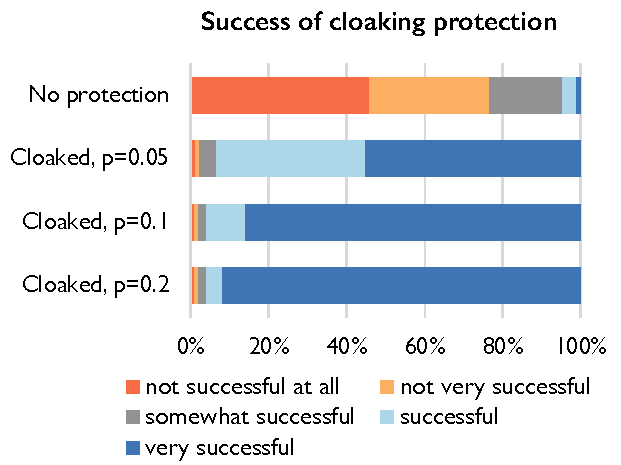
\includegraphics[width=1\columnwidth]{plots/eval/user-cloak-budget.pdf}
  \vspace{-0.23in}
  \caption{\system{}'s cloaking protection success increases as cloak perturbation budget increases. The top row of the figure shows baseline performance with the mimic trains on uncloaked images (p=0). }
  \label{fig:budget-increase}
  \end{minipage}
  \hfill
    \centering
    \begin{minipage}{0.32\textwidth}
  \vspace{0.23in}
  \centering
    \resizebox{1\textwidth}{!}{
    \begin{tabular}{lcc}
    \toprule
    \multicolumn{1}{c}{\textbf{\begin{tabular}[c]{@{}c@{}}Perturbation\\ budget\end{tabular}}} & \textbf{\begin{tabular}[c]{@{}c@{}}Artist-rated \\ PSR\end{tabular}} & \textbf{\begin{tabular}[c]{@{}c@{}}CLIP-based \\ genre shift\end{tabular}} \\ \midrule
    0 (no cloak) & $4.6 \pm 1.4\%$ & $2.4 \pm 0.8\%$ \\
    0.05 & $93.3 \pm 0.6\%$ & $96.0 \pm 0.3\%$ \\
    0.1 & $95.9 \pm 0.4\%$& $98.2 \pm 0.1\%$ \\
    0.2 & $96.1 \pm 0.3\%$ & $98.5 \pm 0.1\%$ \\ \bottomrule
    \end{tabular}
    }
    \vspace{0.13in}
    \captionof{table}{Performance of our system (artist-rated protection success rate and CLIP-based genre shift rate) increases as the perturbation budget increases. (SD model, averaged over all victim artists). }
    \label{tab:budget-increase-sd}
  \end{minipage}
  \hfill
\centering
  \begin{minipage}{0.32\textwidth}
  \centering
  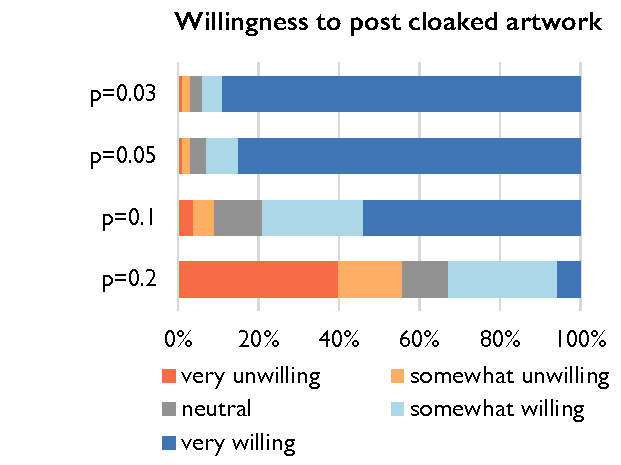
\includegraphics[width=1\columnwidth]{plots/eval/user-accept.pdf}
  \vspace{-0.23in}
  \caption{Artists' willingness to post cloaked artwork in place of the original decreases as perturbation budget of the cloaks increases. }
  \label{fig:artist-accept} 
  \end{minipage}
    \hfill
\end{figure*}

\begin{figure}[t]
  \centering
  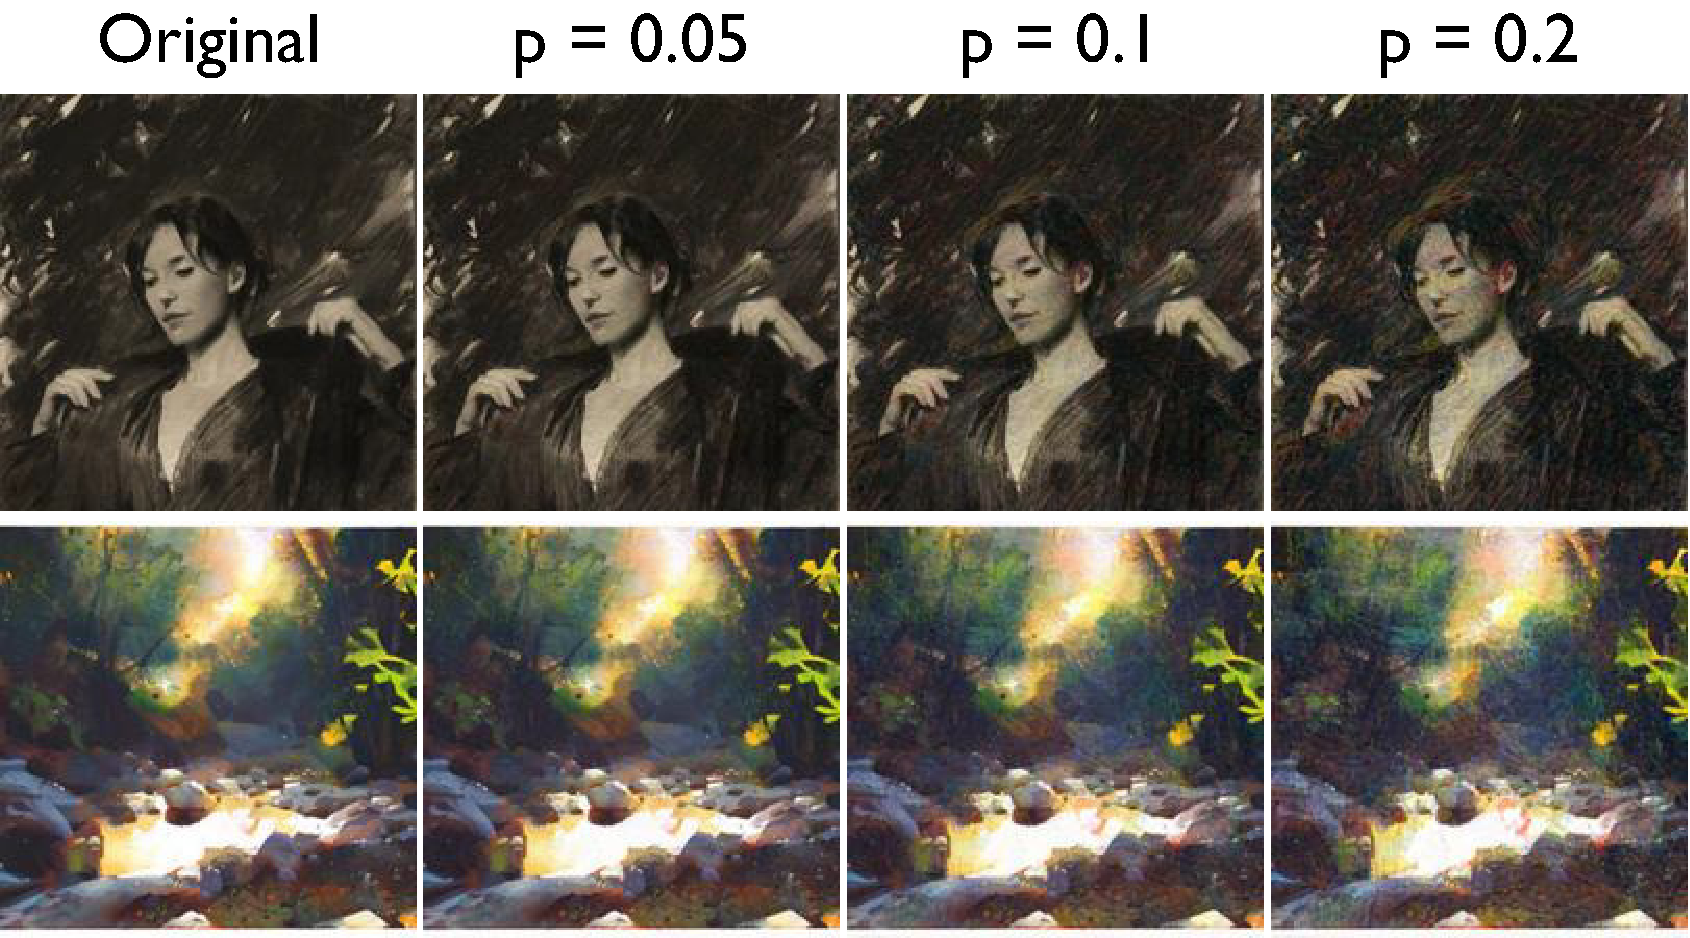
\includegraphics[width=0.90\columnwidth]{plots/eval/cloak-perturbation.pdf}
  \vspace{-0.08in}
  \caption{Original artwork and cloaked artwork computed using three different cloak perturbation budgets. }
  \label{fig:before-after}
\end{figure}

\secspace
\subsection{\system{}'s Protection Performance}
\label{sec:cloaking-results}

\para{Style mimicry success when \system{} is not used. } Mimicry attacks are
very successful when the mimic has access to a victim's original (unmodified)
artwork. Examples of mimicked artwork can be found in
Figure~\ref{fig:core-res}. The leftmost two columns of Figure~\ref{fig:core-res} show a
victim artist's original artwork, while the third column depicts mimicked
artwork generated by a style-specific model trained on victim's original
artwork when \system{} is not used. In our user study, over $>95\%$ of
respondents rated the attack as successful. Table~\ref{tab:psr-core-table},
row 1, gives the artist-rated and CLIP-based genre shift for mimicry attacks on
unprotected art. 

SD models produce stronger mimicry attacks than \dalleM{} models, according
to our user study (see Table~\ref{tab:psr-core-table}). This is unsurprising,
as \dalleM{} models generally produce lower-quality generated
images. CLIP-based genre shift does not reflect this phenomenon, as this metric does
not assess image quality.  

\para{\system{}'s success at preventing style mimicry. } \system{} makes
mimicry attacks markedly less successful, as shown in
Figure~\ref{fig:core-res}. Columns 5 and 6 (from left) show mimicked artwork
when the style-specific models are trained on artwork protected by
\system{}. For reference, column 4 shows an example style-transferred artwork
$\Omega(x, T)$ used to compute \system{} cloaks for the protected art
pieces. Overall, \system{} achieves $> 93.3\%$ artist-rated PSR and
$> 96.0\%$ CLIP-based genre shift (see Table~\ref{tab:psr-core-table}). \system{}'s
protection performance is slightly higher for current artists than for
historical artists. This is likely because the historical artists' images are
present in the training datasets of our generic models (SD, \dalleM),
highlighting the additional challenge of protecting well-known artists whose
style was already learned by the generic models.

\para{How large of perturbations will artists tolerate?} Increasing the
\system{} perturbation budget enhances protection performance. We observe
that both artist-rated and CLIP-based genre shift increase with perturbation budget
(see Figure~\ref{fig:budget-increase}, Table~\ref{tab:budget-increase-sd},
and Figure~\ref{fig:budget2results}). Given this tradeoff between protection
success and \system{} protection visibility on original artwork, we evaluate
how perturbation size impacts artists' willingness to use \system{}. 

We find that artists are willing to add fairly large \system{} perturbations
to their artwork in exchange for protection against mimicry. To measure this,
we show $3$ randomly chosen pairs of original/cloaked artwork to each of the
1,156 artists in our first study. For each art pair, we ask the artist
whether they would be willing to post the cloaked artwork (instead of the
original, unmodified version) on their personal website. More than $92\%$ of
artists select ``willing'' or ``very willing'' when $p=0.05$. This number
only slightly increases to $94.3\%$  when $p=0.03$.
Figure~\ref{fig:artist-accept} details artists' preferences as perturbation
budget increases. (see Figure~\ref{fig:before-after} for examples of cloaked
artwork with increasing $p$). Based on these results, we use perturbation
budget $p = 0.05$ for all our experiments, since most artists are willing to
tolerate this perturbation size.  

Surprisingly, over $32.8\%$ artists are willing to use cloaks with $p=0.2$,
which is clearly visible to human eye (see Figure~\ref{fig:before-after}). While we
are surprised by this high perturbation tolerance, in our follow-up free
response artists noted that they would be willing to tolerate large
perturbations because of the devastating consequence if their styles are
stolen. One participant stated that ``I am willing to sacrifice a bit image
quality for protection.'' Many artists ($>80\%$) also noted that they have
already used traditional, more visually disruptive techniques to protect
their artwork online when posting online, \ie adding watermark or reducing
image resolution. One participant stated that ``I already use low to medium
resolution images only for online posting, thus this would not impact my
quality control too much.'' 

\begin{figure*}[t]
  \centering
  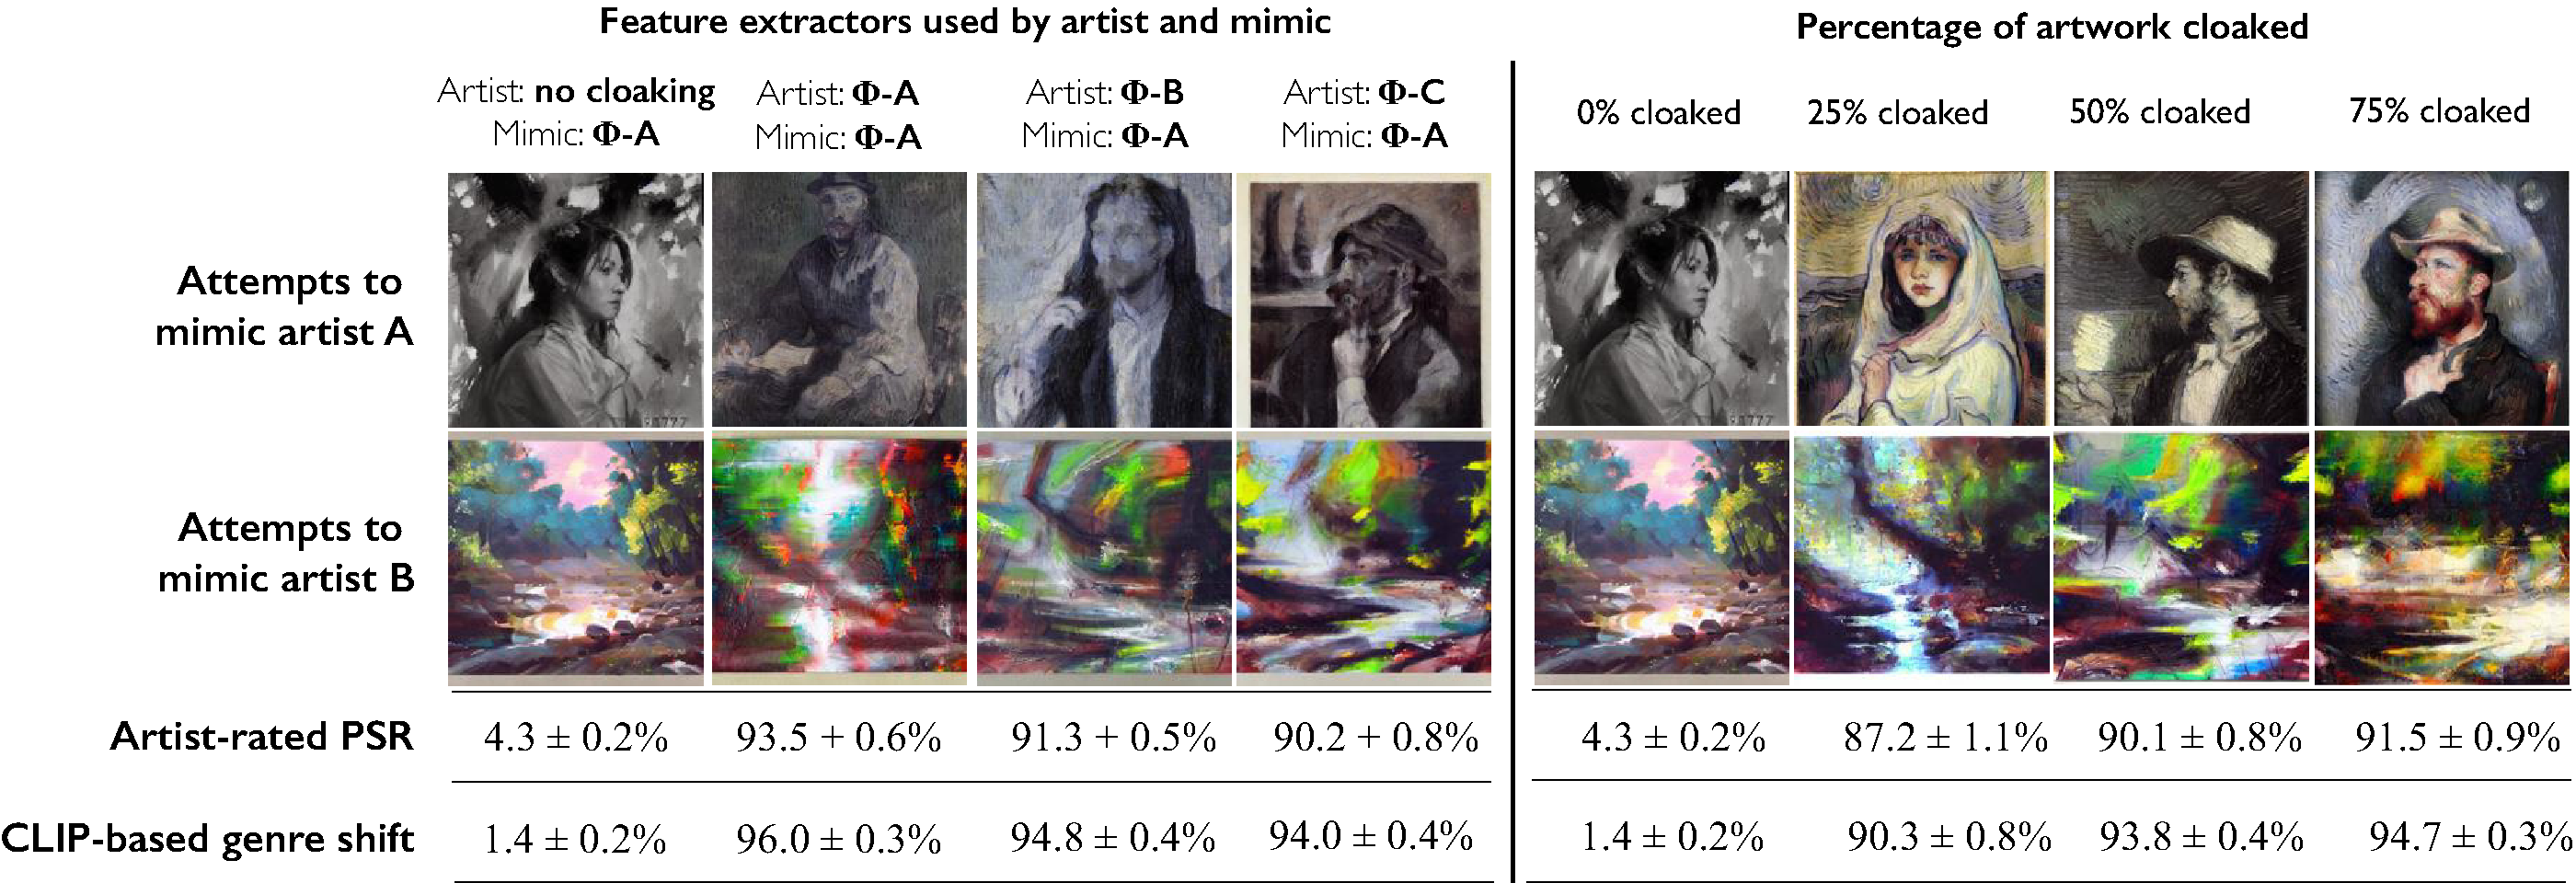
\includegraphics[width=0.95\linewidth]{plots/eval/eval-robust.pdf}
  \caption{\system{} remains successful under two challenging
    scenarios. Left: when artist and mimic use different feature
    extractors. Right: when artists can only cloak a portion of their artwork
    in mimic's dataset. Bottom of the figure shows artist-rated PSR and
    CLIP-based genre shift for the corresponding setting. } 
  \label{fig:core-robust}
\end{figure*}

\secspace
\subsection{\system{}'s Protection Robustness}
\label{sec:robust-eval}

\secspace

Next, we test \system{}'s efficacy in more challenging scenarios. First, we
measure performance when the mimic uses a different feature extractor for
mimicry than the one used by the artist to generate the cloak. Second, we
measure what happens when the mimic has uncloaked artwork samples from the
victim.  Due to the poor mimicry performance of \dalleM, we focus our
evaluation using SD as the generic model.

\para{Artist/mimic use different feature extractors. } In the real world, it
is possible that the mimic will use a different model (and thus a different image
feature extractor) for style mimicry than the one used by the victim artist
to cloak their artwork. While the feature extractors may still be similar
because of the well-known transferability property between large
models~\cite{demontis2019adversarial,transfer,suciu2018does,transfer2014,shan2022post},
their differences could reduce the efficacy of cloaking. We test this
scenario using three feature extractors\textemdash $\Phi$-A, $\Phi$-B, and
$\Phi$-C. $\Phi$-A and $\Phi$-B have different model architectures
(autoencoder-KL~\cite{rombach2022high} vs. VQ-VAE~\cite{ramesh2021zero}) but
are both trained on the ImageNet dataset~\cite{deng2009imagenet}. $\Phi$-A
and $\Phi$-C have different model architectures (autoencoder-KL vs VQ-VAE)
and training datasets (ImageNet vs. CelebA~\cite{liu2018large}).

In our experiments, the victim artist uses one feature extractor (either
$\Phi$-B or $\Phi$-C) to optimize cloaked artwork, and the mimic trains their
style-specific models with SD models using $\Phi$-A. Despite the difference
in victim/mimic extractors, \system{}'s protection remains highly successful
(left half of Figure~\ref{fig:core-robust})\textemdash the style of mimicked
artwork remains distinct from artist's true style. Artist-rated and
CLIP-based genre shift measurements confirm this observation. Artist-rated PSR is
$> 90.2\%$, while CLIP-based genre shift is $> 94.0\%$. The PSR is slightly higher
when the two feature extractors only differ in architectures ($\Phi$-B to
$\Phi$-A) than when they differ in both architecture and training data
($\Phi$-C to $\Phi$-A).


\para{Mimic has access to uncloaked artwork. } Another challenging scenario
is when the mimic gains access to some \textit{uncloaked} artwork from victim
artists. This is a realistic scenario for many prominent artists with a large
online presence. As expected, \system{}'s protection performance decreases
when the mimic has access to more uncloaked artwork (right side of
Figure~\ref{fig:core-robust}). As the ratio of uncloaked/cloaked art in the
mimic's dataset increases, the mimicked artwork becomes more similar to
artist's original style. Yet, \system{} is still reasonably effective
($87.2\%$ artist-rated PSR) even when artists can only cloak $25\%$ of their
artwork. This validates our hypothesis in \S\ref{sec:cloak-effect} that
cloaking will have a noticeable effect as long as the mimic has some cloaked
training data.

A mimic with access to a large amount of uncloaked artwork is still an issue
for \system{}. Fortunately, in our user study, we found that 1) many artists
constantly create and share new artwork online, which can be cloaked to
offset the percentage of uncloaked artwork, and 2) many artists change their
artistic style over time. In our user study, we asked artists to estimate the
number of unique art pieces they currently have online ($M$) and the
estimated number of art pieces they anticipate uploading each subsequent year
($Y$). Among artists with an existing online presence, over $40\%$ have
$Y / M > 25\%$, meaning that one year from now, $> 20\%$ of their total
online artwork would be cloaked (if they start using \system{}
immediately). More than $81\%$ of artists also stated that their art style
has changed over their career, and half of these said that theft of their
old, outdated styles is less concerning.


\begin{table}[t]
  \centering
  \resizebox{0.49\textwidth}{!}{
  \centering
  \begin{tabular}{ccccc}
    \hline
    \multirow{2}{*}{\textbf{\begin{tabular}[c]{@{}c@{}}Artist \\ dataset\end{tabular}}} & \multicolumn{2}{c}{\textbf{w/o \system}} & \multicolumn{2}{c}{\textbf{w/ \system{} (p=0.05)}} \\ \cline{2-5} 
     & \begin{tabular}[c]{@{}c@{}}Artist-rated \\ PSR\end{tabular} & \begin{tabular}[c]{@{}c@{}}CLIP-based \\ genre shift\end{tabular} & \begin{tabular}[c]{@{}c@{}}Artist-rated \\ PSR\end{tabular} & \begin{tabular}[c]{@{}c@{}}CLIP-based \\ genre shift\end{tabular} \\ \hline

    Current & $6.2 \pm 0.5\%$ & $3.8 \pm 0.3\%$ & $92.5 \pm 0.5\%$ & $94.2 + 0.3\%$ \\
    Historical & $7.2 \pm 0.6\%$ & $3.3 \pm 0.4\%$ & $92.1 + 0.3\%$ & $93.9 + 0.4\%$ \\ 
    \hline
    \end{tabular}
  }
  \vspace{-0.1in}
  \caption{Performance of \system{} against real-world mimicry service
    (scenario.gg). Mimicry service achieves high mimicry success when no
    protection is used. When \system{} is used, the mimicry service has low
    performance. }
  \label{tab:real-world}
\end{table}

\secspace
\subsection{Real-World Performance}

Next, we test \system{} against a real-world style mimicry-as-a-service
system, \texttt{scenario.gg}~\cite{aigame}. Scenario.gg is a web service that
allows users to upload a set of images in a specific style. The
service then trains a model to mimic the style and returns an API endpoint
that allows the user to generate mimicked images in the trained style. The
type of model or mimicry method used by the service is unknown.

\system{} remains effective against \texttt{scenario.gg}. We ask
\texttt{scenario.gg} to mimic the style from a set of cloaked or uncloaked
artwork from $4$ current artists and $19$ historical
artists. Table~\ref{tab:real-world} shows that when no protection is used,
\texttt{scenario.gg} can successfully mimic the victim style (< 7.2\%
protection success). The mimicry success of \texttt{scenario.gg} is lower
than our mimicry technique, likely because \texttt{scenario.gg} trains the
model for fewer iterations due to computational constraints. When we use
\system{} to cloak the artwork and upload the cloaked artwork,
\texttt{scenario.gg} fails to mimic the victim style ($> 92.1\%$ artist-rated
PSR and $> 93.9\%$ CLIP-based genre shift rate) as shown in Table~\ref{tab:real-world}.


\section{Scene Splitting Adaptive Attack}
\label{sec:counter}

\system~ removes uncontrolled randomness in perturbations between similar
frames, thereby disabling adaptive attacks that leverage cross frame pixel
correlations. However, does its own design give rise to new countermeasures?
We carefully considered this question, and discuss what we consider the
strongest possible countermeasure to \system{}. We describe the potential
countermeasure and evaluate its efficacy against \system.

The intuition for the countermeasure is to manipulate the scene
identification process to force a scene break between highly similar
frames. If this can be achieved, then the attacker could obtain two
consecutive (and similar) frames that have been perturbed towards different
targets. They could then apply a version of the pixel-averaging attack to
restore the original, unprotected frames. We call this the scene-splitting
attack, and assume a powerful attacker who can somehow force \system{} to
insert a scene break in the middle of a sequence of similar frames.

\para{The scene splitting attack.} 
We simulate a strong adaptive attack by dividing a single scene from a
video into two subscenes, Scene $S_1$ and $S_2$ each containing $M$ frames. We
use each subscene (Scene$_i$) to generate a target tensor $T_{i}$ with the
aim of maximizing distance between target tensors, which should maximize the
difference between perturbations generated from these targets. 
Now that we have obtained $T_1, T_2$, we apply \system~ to perturb the two
consecutive frames around the bad scene split. Subsequently, we perform a
pixel averaging attack on these two perturbed frames, following the
implementation detailed in \S\ref{sec:eval-limitations}. 

We test our adaptive attack on 20 videos from the Japanese Anime and Video
Game datasets (10 videos from each dataset). We choose these two datasets
because they are best aligned with current threats as explained in
\S\ref{sec:intro}. We limit ourselves to only 10 videos from each category
because of the computation time involved.


\begin{figure}[t]
  \centering
  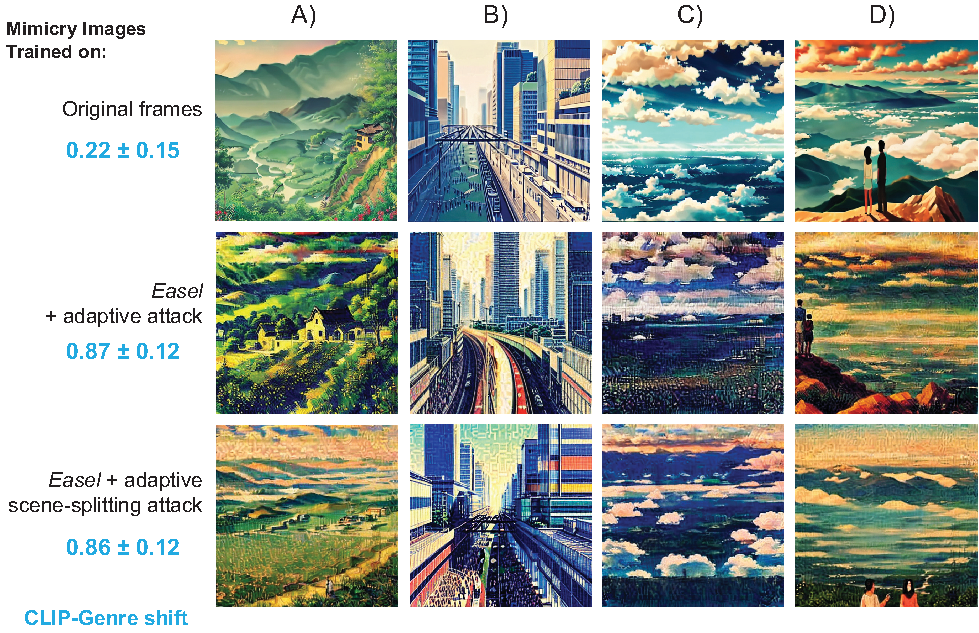
\includegraphics[width=1\columnwidth]{plots/countermeasures-eps-converted-to.pdf}
  \caption{Visual examples of mimicry attempts on Clean frames and frames
    protected by \system~ across the standard Adaptive Attack and the
    Scene-Splitting Adaptive Attack. CLIP-Genre Shift score demonstrates
    robust protection against Mimicry attacks under both adaptive attack
    scenarios.} 
  \label{fig:style-mimicry-ctr}
\end{figure}

\para{\system~ is robust to scene-splitting attack.}
Tables~\ref{tab:countermeasure-loss-score}
and~\ref{tab:countermeasure-pd-score} show results that quantify the
image-level difference between the original frames and the frames produced by
the scene-splitting attack. They show that \system~ is robust to the
scene-splitting attack combined with pixel averaging attacks attempting to
recover original frames. There is only a minimal decrease in $L_2$ norm and
$MPD$ value when \system~ is applied to videos under the new Adaptive
Scene-Splitting Attack. In Figure~\ref{fig:style-mimicry-ctr}, we 
further verify that style mimicry using a combination of
scene-splitting and pixel-averaging is still unsuccessful, through both
visual examples of generated images and associated CLIP-genre shift scores,
which remain unchanged under the scene splitting attack.

\para{Why does the attack fail?} The failure of the scene-splitting attack
makes sense, once we consider its limitations. Regardless of where the
attacker forces a new scene break, frames inside the two new scenes ($S_1$
and $S_2$) are bounded in their maximum difference from each other. Thus the
two source frames for $S_1$ and $S_2$ (each computed as an average of frames
in the scene) is also bounded in their dissimilarity. Thus, it is likely
their resulting target tensors, and consequently the perturbations generated
from them, are also small. This intuition holds even if the attacker could
break a single long scene into several scenes of their choosing.

  \begin{table}[t]
    \centering
      \resizebox{0.5\textwidth}{!}{
      \centering
  \begin{tabular}{c|ccc}
    & Naive         & \multicolumn{1}{c}{\begin{tabular}[c]{@{}c@{}}\system\\ + Adaptive Attack\end{tabular}} & \multicolumn{1}{c}{\begin{tabular}[c]{@{}c@{}}\system~  + Adaptive \\ Scene-Splitting Attack\end{tabular}} \\ \hline
    Video Game     & 405.38 $\pm$ 19.43 & 421.21 $\pm$ 25.52 & 394.80 $\pm$ 25.16       \\
    Japanese Anime & 396.76 $\pm$ 19.05 & 406.43 $\pm$ 24.07 & 387.06 $\pm$ 23.98
\end{tabular}
    }\caption{Latent $L_2$ norm between original and perturbed frames across Video Games and Japanese Anime datasets. Demonstrates Scene-Splitting Adaptive Attack is not able to significantly reduce protection \system~ offers.}
  \label{tab:countermeasure-loss-score}
  \end{table}

  \begin{table}[t]
    \centering
      \resizebox{0.5\textwidth}{!}{
      \centering
  \begin{tabular}{c|ccc}
    & Naive         & \multicolumn{1}{c}{\begin{tabular}[c]{@{}c@{}}\system\\ + Adaptive Attack\end{tabular}} & \multicolumn{1}{c}{\begin{tabular}[c]{@{}c@{}}\system~  + Adaptive \\ Scene-Splitting Attack\end{tabular}} \\ \hline
    Video Game     & 111.58 $\pm$ 12.38 & 107.42 $\pm$ 13.47 & 100.28 $\pm$ 11.81 \\
    Japanese Anime & 112.66 $\pm$ 11.05 & 108.57 $\pm$ 12.59 & 102.02 $\pm$ 11.43       
\end{tabular}
    }\caption{MPD between original and perturbed frames across Video Games and Japanese Anime datasets. Demonstrates Scene-Splitting Adaptive Attack is not able to significantly reduce protection \system~ offers.}
  \label{tab:countermeasure-pd-score}
  \end{table}



We explored LLMs and their alignment with neural responses during language processing, uncovering several key findings. Firstly, we observed a clear correlation between the language task performance of LLMs and their accuracy in predicting neural responses in the auditory cortex, with higher-performing models exhibiting greater functional alignment with the speech cortex. Secondly, we showed that the models with higher performance on benchmark tasks achieved peak predictive accuracy in earlier layers. In contrast, lower-performing models exhibited a delayed representation, necessitating deeper layers to approach similar levels of brain prediction accuracy. Finally, our study highlights the crucial role of contextual information in both LLMs and brain processing, where the contextual window's size significantly influenced the difference between better and worse models, with the availability of long-range contextual information driving the high-performing LLMs closer to the brain's hierarchical pathway. These findings uncover fundamental principles in language processing, highlighting the critical role of hierarchical structure and contextual dependencies in language which give rise to convergent processing strategies in both artificial and biological systems. 

\subsection{Hierarchical Processing and Inter-Model Comparisons}
We found that better-performing LLMs exhibit a more brain-like hierarchy of layers, offering new insights into their language processing. While previous studies have revealed similarities in the hierarchical stages found in the brain and deep neural networks for linguistic \cite{caucheteux2023evidence, caucheteux2022brains, kumar2022reconstructing}, acoustic \cite{giordano2023intermediate, tuckute2023many}, visual \cite{kriegeskorte2015deep, cichy2016comparison, sexton2022reassessing}, and imagined stimuli \cite{horikawa2017hierarchical}, a distinct approach in our study is the inter-model comparison within a consistent architectural framework. In related work analyzing deep neural networks for vision tasks, recent evidence \cite{nonaka2021brain} has shown that better performance can create a less brain-like progression of feature extraction in models when compared to the visual cortex, suggesting that the complex architectures of high-performing image processing networks have steered them away from neural alignment. By examining LLMs based on a single architecture, the stacked transformer decoder \cite{vaswani2017attention}, we uncover differences in their alignment with the brain's hierarchical stages during language comprehension. Transformer language models use contextual features to encode linguistic, syntactic, and positional structures \cite{o2021context, clark2019does}, and increasingly high-level and context-specific features arise throughout a model’s layers \cite{ethayarajh2019contextual, tenney2019bert}. This may be partly because later layers bind linguistic structures over longer contexts \cite{skrill2023large}. The crucial observation that such models display brain-like hierarchies resonates with neurobiological findings of hierarchical organization in the auditory and language-related cortex \cite{hickok2007cortical, sharpee2011hierarchical, sheng2019cortical, ding2017characterizing, hasson2008hierarchy, lerner2011topographic, norman2022multiscale, de2017hierarchical}. The convergence of the two systems highlights language's inherent hierarchical structure as we increasingly form larger units of representation, from articulatory features to phonemes, syllables, words, sentences, and phrases \cite{keshishian2023joint, di2021neural, gong2023phonemic}. Our results demonstrate that as LLMs have achieved higher performance, they have done so using feature extraction pathways that more closely resemble the human brain.

\subsection{Feature Extraction Efficiency and Contextual Processing}
A significant finding of our study is the delayed feature extraction observed in less effective LLMs compared to their higher-performing counterparts. This delay, particularly evident in the early processing stages within transformer models, suggests a slower buildup of relevant linguistic and contextual information \cite{tenney2019bert}. The implications of this observation are multifaceted. Firstly, it challenges the conventional emphasis on the final layers of LLMs \cite{goldstein2022shared}, instead drawing attention to the critical role of initial layers in efficient language processing \cite{antonello2023predictive}. This shift in focus aligns with emerging neuroscience research that underscores the significance of early-stage processing in the human brain for complex cognitive tasks like language processing \cite{de2017hierarchical, keshishian2023joint, gong2023phonemic}. Secondly, this delayed representation in less effective models offers insights into potential inefficiencies in their training or design. Given the architectural similarity of models in our study, the variance in feature extraction efficiency among models may reflect differences in training strategies \cite{naveed2023comprehensive} and data quality \cite{raffel2020exploring, lee2021deduplicating, touvron2023llama2}, providing insights for future LLM model development. As LLMs have evolved in recent years, improvements in dataset size and cleanliness as well as architectural changes to increase context length have come along with their performance improvements, and our results show that these improvements have also given rise to greater brain similarity. Furthermore, the observation that higher-performing models utilize early layers more effectively and peak in their brain similarity in middle layers rather than later layers raises intriguing questions about the role of subsequent layers. It is possible that these later layers are engaged in next-level contextual integration and feature extraction, potentially analogous to higher-order stimulus integration to support cognitive functions in the human brain \cite{huth2016natural, murphy2023spatiotemporal}. Alternatively, this finding could point to a limitation in our current methodologies, such as limited iEEG coverage, the simplicity of the speech comprehension task, or the fact that LLMs are not explicitly trained to perform comprehension, but rather next-word prediction, which is slightly different from the speech listening comprehension task the subjects performed. Our iEEG recordings include broad coverage of speech processing regions, especially acoustic sensory regions like HG and STG, which, although critical for spoken language processing, represent a slightly different aspect of linguistic feature extraction than the token-level processing that transformer architecture LLMs begin with. Answering these questions is crucial for enriching our understanding of artificial language processing.

The influence of contextual information on brain similarity and LLM benchmark scores also points to specific avenues that may improve model performance on language tasks. Ensuring that models are able to extract long context windows, such as by using architectures that allow for long context windows \cite{xiong2023effective} and utilizing training data that is rich in long context information, could enhance LLM performance further beyond simply scaling up a model's parameter size. Transformer-based LLMs have been shown to suffer from unequal contextual information extraction when the prior context occurs at different distances from the target \cite{liu2023lost}, supporting the notion that improving the robustness of modern LLMs to varying context lengths may lead to performance improvements. Our investigation offers a unique lens through which to view the parallels and divergences between machine learning and human cognitive development.

\subsection{Convergence to Brain-Like Models for Human-Level Artificial General Intelligence}

The convergence of LLMs and human speech processing may suggest that certain fundamental principles underlying efficient language processing might be common to both artificial and biological systems. The human brain's language capabilities have developed as an adaptive response to complex communication needs, optimizing for efficiency and versatility \cite{pinker1990natural}. Our findings suggest that LLM architectures and processing strategies are gravitating towards these same principles, mimicking the brain’s evolutionary adaptations for language. LLMs are trained without consideration for brain similarity, yet they have become increasingly brain-like in their feature extraction and hierarchical processing. Brain-like processing may represent an optimal solution to language modeling found by evolution \cite{deacon1997symbolic}, although subject to biological constraints, and our results suggest that modern LLM training focused on performance optimization may have placed these models on a similar path. In our study, Mistral, the top-performing model, stands as a prime example of this convergence, where the degree of similarity of a model’s embeddings to those of Mistral is highly correlated with performance and brain similarity. This evolution towards an optimal brain-like model offers an intriguing suggestion regarding artificial general intelligence (AGI). While not clearly defined, AGI can be quantified as human-level performance on a broad set of benchmarks \cite{goertzel2014artificial}. Our findings suggest that developing models mimicking human neural processing strategies \cite{zhao2023brain}, rather than solely focusing on augmenting computational power or diversifying learning algorithms \cite{zhao2023survey}, could accelerate the development of models that behave on par with human performance. Hence, brain similarity could be a useful evaluation and optimization metric for future model development.

Our research marks a significant stride in understanding the parallels between large language models and human brain processes in language comprehension, by revealing the intricate relationship between internal model representation, model performance, and neural predictive accuracy. Our findings enhance the understanding of LLMs and offer new insights into the cognitive mechanisms underlying human language processing. 


% Our study reveals a compelling trend: the better an LLM performs, the more it resembles both the structure and function of the human brain and other high-performing LLMs. In particular, Mistral, the top-performing model, stands as a prime example of this convergence, where the degree of similarity of a model's embeddings to those of Mistral is highly correlated with the performance and, accordingly, the brain similarity. This trend suggests a significant correlation between the performance of a model, its similarity to brain processes, and its internal representation and processing of information.

% The evolution towards an optimal brain-like model has significant implications for artificial general intelligence (AGI). Recent renewed focus on the creation of AGI spans many domains, and AGI itself is hard to define, often being defined based on high performance on broad benchmark tests and considered differently from human-level AGI, another loose term referring to AI that matches human performance \cite{goertzel2014artificial}. Here, we restrict our focus to the creation of human-level AGI models. Given our findings, achieving human-level AGI might be realized by developing models that mimic human neural processes \cite{zhao2023brain}, since similarity to human language processing pathways is highly related with performance, despite brain similarity never being explicitly used when training these models. This observation underscores a strategic pivot in the pursuit of AGI. Rather than solely focusing on augmenting computational power or diversifying learning algorithms \cite{zhao2023survey}, an emphasis on developing models that mirror the neural architectures and processing strategies of the human brain could be the key to achieving human-level AGI. Brain similarity could be a useful evaluation metric for future models, enabling the field to understand how close a model is to something human-level.

% Such a strategy is supported by findings in neuroscience and cognitive science, which have long suggested that the human brain architecture offers efficient solutions to complex cognitive tasks \cite{deacon1997symbolic}. Our research marks a significant stride in understanding the parallels between large language models and human brain processes in language comprehension, by revealing the intricate relationship between internal model representation, model performance, and neural predictive accuracy. The correlation between high-performing LLMs and brain-like processing indicates that the most advanced AI systems may naturally evolve toward architectures that resemble human cognition, both behavior-wise and system-wise. Our findings enhance the understanding of LLMs and offer new insights into the cognitive mechanisms underlying human language processing.





% \red{Our study reveals a compelling trend: the better a LLM performs, the more it resembles both the structure and function of the human brain and other high-performing LLMs. In particular, Mistral, the top-performing model, stands as a prime example of this convergence, where the degree of similarity of representations to Mistral's is highly correlated with the performance and, accordingly, the brain similarity. This trend suggests a significant correlation between the performance of a model, its similarity to brain processes, and its internal representation and processing of information. This correlation implies that an optimal model in terms of performance also entails the most brain-like processing such a model can obtain.}

% \red{The evolution towards an optimal brain-like model has significant implications for artificial general intelligence (AGI). If the highest level of LLM performance equates to a model that functions similarly to the human brain, it implies that achieving AGI, a system capable of performing any human cognitive task, could be realized by developing models that mimic human neural processes \cite{zhao2023brain}. This observation underscores a strategic pivot in the pursuit of AGI. Rather than solely focusing on augmenting computational power or diversifying learning algorithms \cite{zhao2023survey}, an emphasis on developing models that mirror the neural architectures and processing strategies of the human brain could be the key to achieving true AGI. This approach aligns with the principle that the most efficient and effective solutions to complex problems like natural language processing may already exist in the natural world, particularly in the form of human cognitive processes \cite{bar2011biomimetics}.}

% \red{Such a strategy is supported by findings in neuroscience and cognitive science, which have long suggested that human brain architecture offers efficient solutions to complex cognitive tasks \cite{deacon1997symbolic}. The correlation between high-performing LLMs and brain-like processing indicates that the most advanced AI systems may naturally evolve toward architectures that resemble human cognition, both behavior-wise and system-wise. Our findings highlight a potential path to AGI through the development of brain-like models. This approach not only promises improvements in AI performance by achieving brain-like information processing but also aligns AI development with the sophisticated and efficient design of the human brain, offering a promising direction for future research in AI and cognitive science.}

{
 \footnotesize
 \bibliographystyle{acm}
 \bibliography{glaze}
}

\balance

\appendix
\appendix

% \section{Claimed Emergent Abilities}
% \label{app:claimed_emergent_abilities}

% We compile the models, tasks and metrics that different papers have claimed reveal emergent abilities of large language models. This list may be incomplete or inaccurate, but represents a good faith attempt to compile this information. Note: quantifying model scale when an ability emerges is complicated by the fact that different papers report model scale differently, either as (a) number of parameters \cite{brown2020language, ganguli2022predictability}, (b) effective number of parameters \cite{srivastava2022beyond} or (c) training FLOPs \cite{wei2022emergent}.

% \begin{table}[h!]
%     \centering
%     \begin{tabular}{|l|c|c|c|}
%     \hline
%         Task & Model Families & Metric & Model Scale at Emergence \\
%         \hline
%         2-Digit Addition \cite{brown2020language} & GPT-3 & Accuracy & 13B Parameters\\
%         2-Digit Subtraction \cite{brown2020language} & GPT-3 & Accuracy & 13B Parameters\\
%         3-Digit Addition \cite{brown2020language, ganguli2022predictability} & GPT-3 & Accuracy & 175B Parameters\\
%         3-Digit Subtraction \cite{brown2020language} & GPT-3 & Accuracy & 175B Parameters\\
%         MMLU \cite{ganguli2022predictability} & GPT-3, Gopher & Accuracy & 200B, 300B Parameters\\
%         Program Synthesis \cite{ganguli2022predictability} & Google Internal & \% Samples Solving Task & 200B Parameters\\
%         Figure of Speech Detection \cite{srivastava2022beyond} & ? & ? & $\sim 10^{11}$ Effective Parameters \\
%         IPA Transliterate \cite{srivastava2022beyond, wei2022emergent} & LaMDA, GPT-3 & BLEU & $\sim 10^{23}, \sim 10^{23}$ Training FLOPs\\
%         Periodic Elements \cite{srivastava2022beyond} & ? & ? & ?\\
%         Modified Arithmetic \cite{srivastava2022beyond, wei2022emergent} & GPT-3, LaMDA & Accuracy & $\sim 10^{23}, \sim 10^{24}$ Training FLOPs\\
%         Repeat Copy Logic \cite{srivastava2022beyond} & ? & ? & $10^{11}$ Effective Parameters\\
%         Word Unscrambling \cite{srivastava2022beyond, wei2022emergent} & LaMDA & Exact Match & $\sim 10^{24}$ Training FLOPs\\
%         Persian QA \cite{wei2022emergent} & PaLM & Exact Match & $\sim 10^{24}$ Training FLOPs\\
%         Truthful QA \cite{wei2022emergent} & Gopher & Accuracy & $\sim 10^{23}$ Training FLOPs\\
%         Grounded Mappings \cite{wei2022emergent} & ? & ? & ?\\
%         Multi-task NLU \cite{wei2022emergent} & ? & ? & ?\\
%         Word in context \cite{wei2022emergent} & ? & ? & $\sim 10^{24}$ Training FLOPs\\
%         \hline
%     \end{tabular}
%     \newline
%     \caption{\textbf{Tasks, model families, metrics and number of parameters for emergent abilities.}}
%     \label{tab:my_label}
% \end{table}


% \section{Exponentiated Negative Cross Entropy Lower Bounds Accuracy}
% \label{app:acc_bound}

% Consider batch size $B$ with length $L$. During training i.e. with teacher-forcing, the per-token accuracy (averaged over batch index $b$ and sequence index $l$) is defined as:
% %
% \begin{align}
%     \text{Acc} &\defeq \frac{1}{B} \sum_b \frac{1}{L} \sum_l p(t_{bl}^* | t_{b, <l}^*)\\
%     &= \frac{1}{BL} \sum_{b, l} p(t_{bl}^* | t_{b, <l}^*)
% \end{align}

% The cross entropy (commonly averaged over the batch) is defined as:
% %
% \begin{align}
%     \mathcal{L}_{CE} &\defeq -\frac{1}{B} \sum_b \log p(t_{b 1}^*, ..., t_{b L}^*)\\
%     &= -\frac{1}{B} \sum_b \log \prod_l p(t_{b l}^*| t_{b, <l}^*)\\
%     &= -\frac{1}{B} \sum_{b, l} \log p(t_{bl}^* | t_{b, <l}^*)
% \end{align}

% To make the comparison between accuracy and cross entropy a little easier, let's normalize the cross entropy by the sequence length:
% %
% \begin{align}
%     \mathcal{L}_{CE/L} &\defeq \frac{1}{L}\mathcal{L}_{CE}\\
%     &=  -\frac{1}{BL} \sum_{b, l} \log p(t_{bl}^* | t_{b, <l}^*)
% \end{align}

% Recall that Jensen's inequality tells us that for any random variable $X$, $\log \mathbb{E}[X] \geq \mathbb{E}[\log X]$. The relationship between sequence-length-normalized cross entropy and accuracy is thus:
% %
% \begin{align}
%     -\mathcal{L}_{CE/L} = \frac{1}{BL} \sum_{b, l} \log p(t_{bl}^* | t_{b <l}^*) &\leq \log \frac{1}{BL} \sum_{b, l}  p(t_{bl}^* | t_{b <l}^*) = \log \text{Acc}\\
%     \exp(- \mathcal{L}_{CE/L}) &\leq \text{Acc}
% \end{align}

% Consequently, we see that driving the cross entropy loss to $0$ necessarily drives the accuracy to $1$.

% TODO: Can we use the second moment method to derive bounds on how (un)likely a subset of tokens are to deviate from the mean?


\section{Approximate Behavior of Metrics on Sequential Data}
\label{app:metric_scaling}

How do different metrics behave when used to measure autoregressive model outputs? Precisely answering this question is tricky and possibly analytically unsolvable, so we provide an approximate answer here.

Notationally, we consider $N$ test data of length $L$ (here, length is measured in tokens) with targets denoted $t_n \defeq (t_{n1}, t_{n2}, ... t_{nL})$, the autoregressive model has a true-but-unknown per-token error probability of $\epsilon \in [0, 1]$ and the model outputs prediction $\hat{t}_n \defeq (\hat{t}_{n1}, \hat{t}_{n2}, ... \hat{t}_{nL})$. This assumes that the model's per-token error probability is constant, which is empirically false, but modeling the complex dependencies of errors is beyond our scope.

\subsection{Per-Token Error Probability is Resolution-Limited}
\label{app:metric_scaling:resolution_limited}

Note that because we have $N$ test data, each of length $L$, our resolution for viewing the per-token error probability $\epsilon$ is limited by $1/NL$. 
Here, resolution refers to ``the smallest interval measurable by a scientific instrument; the resolving power."
To explain what resolution means via an example, suppose one wants to measure a coin's probability of yielding heads.
After a single coin flip, only two outcomes are possible (H, T), so the resolution-limited probability of heads is either $0$ or $1$.
After two coin flips, four outcomes are possible (HH, HT, TH, TT), so the resolution-limited probability of heads is now one of $0, 0.5, 1$.
After $F$ coin flips, we can only resolve the coin's probability of yielding heads up to $1/F$.
Consequently, we introduce a resolution-limited notation:
%
\begin{equation}
    \nint{a}_b \defeq \text{$a$ rounded to the nearest integer multiple of $1/b$}
\end{equation}

\subsection{Token Edit Distance}
\label{app:metric_scaling:token_edit_distance}

We first consider an adaptation of the Levenshtein (string edit) distance for models that function on tokens rather than characters, an adaptation we term the \textit{token edit distance}. The token edit distance between two token sequences $t_n, \hat{t_n}$ is defined as the integer number of additions, deletions or substitutions necessary to transform $t_n$ into $\hat{t}_n$ (or vice versa).

\begin{align}
    \text{Token Edit Distance}(t_n, \hat{t}_n)  &\defeq \text{Num Substitutions} + \text{Num. Additions} + \text{Num. Deletions}\\
    &= \sum_{\ell =1}^L \mathbb{I}[t_{n\ell} \neq \hat{t}_{n\ell}] + \text{Num. Additions} + \text{Num. Deletions}\\
    &\geq \sum_{\ell =1}^L \mathbb{I}[t_{n\ell} \neq \hat{t}_{n\ell}]
\end{align}

The expected token edit distance is therefore:

\begin{align}
    \mathbb{E}[\text{Token Edit Distance}(t_n, \hat{t}_n)] &\geq \mathbb{E}[\sum_{\ell =1}^L \mathbb{I}[t_{n\ell} \neq \hat{t}_{n\ell}]]\\
    &= \sum_{\ell =1}^L p(t_{n\ell} \neq \hat{t}_{n\ell})\\
    &\approx L (1 - \epsilon)
\end{align}

The resolution-limited expected token edit distance is therefore:

\begin{equation}
    \nint{\mathbb{E}[\text{Token Edit Distance}(t_n, \hat{t}_n)]}_{NL} \geq L \Big(1 - \nint{\epsilon}_{NL} \Big)
\end{equation}

From this, we see that the expected token edit distance scales approximately linearly with the resolution-limited per-token probability. The real rate is slightly higher than linear because additions and deletions contribute an additional non-negative cost, but modeling this requires a model of how likely the model is to overproduce or underproduce tokens, which is something we do not currently possess.

\subsection{Accuracy}
\label{app:metric_scaling:accuracy}

\begin{align}
    \text{Accuracy}(t_n, \hat{t}_n) &\defeq \mathbb{I}[\text{No additions}] \, \mathbb{I}[\text{No deletions}] \, \prod_{l=1}^L \mathbb{I}[t_{nl} = \hat{t}_{nl}]\\
    &\approx \prod_{l=1}^L \mathbb{I}[t_{nl} = \hat{t}_{nl}]
\end{align}

As with the Token Edit Distance (App. \ref{app:metric_scaling:accuracy}), we ignore how likely the language model is to overproduce or underproduce tokens because we do not have a good model of this process. Continuing along,

\begin{align}
    \mathbb{E}[\log \text{Accuracy}] &= \sum_l \mathbb{E}[\log \mathbb{I}[t_{nl} = \hat{t}_{nl}]]\\
    &\leq \sum_l \log \mathbb{E}[\mathbb{I}[t_{nl} = \hat{t}_{nl}]]\\
    &\approx L \log (1- \epsilon)
    % \exp(\mathbb{E}[\log \text{Accuracy}]) &= \exp (\sum_l \mathbb{E}[\log \mathbb{I}(t_{nl}, \hat{t}_{nl})])\\
    % &=
\end{align}

Taking an approximation that would make most mathematicians cry:

\begin{align}
    \mathbb{E}[\text{Accuracy}] &\approx \exp(\mathbb{E}[\log \text{Accuracy}])\\
    &= (1 - \epsilon)^L\\
\end{align}

This reveals that accuracy \textbf{approximately} falls geometrically with target token length. The resolution-limited expected accuracy is therefore:

\begin{equation}
    \nint{\mathbb{E}[\text{Accuracy}]}_{NL} = \nint{(1 - \epsilon)^L}_{NL}
\end{equation}

From this we can see that choosing a nonlinear metric like Accuracy is affected significantly more by limited resolution because Accuracy forces one to distinguish quantities that decay rapidly.

\subsection{ROUGE-L-Sum}
\label{app:metric_scaling:rougeLsum}

\begin{figure}
    \centering
    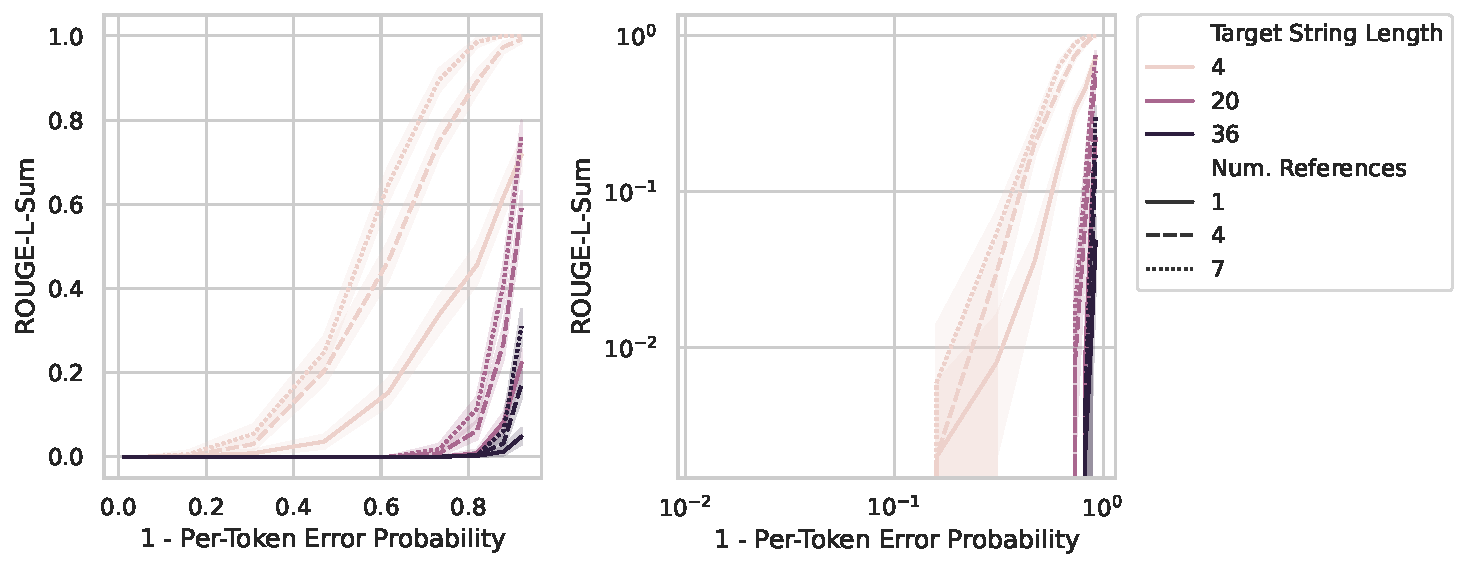
\includegraphics[width=0.95\textwidth]{figures/rouge_understanding/rougeLsum_vs_token_error_prob_scaling_simulation.pdf}
    \caption{\textbf{ROUGE-L-Sum is a sharp metric.} Simulations show that as the per-token error probability slightly increase (e.g. from 0.05 to 0.1), the ROUGE-L-Sum metric sharply falls.}
    \label{fig:app:metric_scaling:rougeLsum}
\end{figure}


Another BIG-Bench metric \cite{srivastava2022beyond} is ROUGE-L-Sum \cite{lin2004rouge}, a metric based on the longest common subsequence (LCS) between two sequences. Section 3.2 of \cite{lin2004rouge} gives the exact definition, but the key property is that ROUGE-L-Sum measures the ``union" LCS, which means ``stitching" together LCSs across the candidate and multiple references. As explained in the original paper: if the candidate sequence is $c = w_1 w_2 w_3 w_4 w_5$, and if there are two reference sequences $r_1 = w_1 w_2 w_6 w_7 w_8$ and $r_2 = w_1 w_3 w_8 w_9 w_5$, then $LCS(r_1, c) = w_1 w_2$ and $LCS(r_2, c) =w_1 w_3 w_5$, then the \textit{union} 
-LCS of $c, r_1, r_2$ is $w_1 w_2 w_3 w_5$, with length 4. Intuitively, this disproportionately benefits models with smaller error rates because their mistakes can be ``stitched" across multiple references; this is confirmed in simulation (Fig. \ref{fig:app:metric_scaling:rougeLsum}).


% \subsection{BLEU}
% \label{app:metric_scaling:bleu}


% \subsection{Emergence does not require on scaling laws: decreasing cross-entropy loss and stricter exact match is all you need }

% The goal of this section is to show that scaling laws are not necessary to create emergence and that many functional forms of the loss are valid as long as the form decreases as some other variable decreases -- say the number of parameters in the model.
% This typically holds in modern machine learning. 
% We do this by considering different functional forms of the cross entropy $CE(N)$, as a function of the number of parameters $N$, and show emergence, i.e. sharpness and unpredictability.
% We illustrate this by showing the programmer can exaggerate the sharpness (and therefore emergence) by implying increasing the exact number of tokens required to get correct in the accuracy, i.e. increasing $L$ in our notation.

% \subsubsection{Argument}

% Recall from section \ref{sec:alt_explanation} the accuracy requiring all $L$ tokens to be correct for a model of size $N$ as a function of cross-entropy $CE(N)$:

% \begin{equation*}
%     \text{Accuracy}(N) \approx p_N(\text{single token correct})^{\text{num. of tokens}} = \exp \Big(- CE(N) \Big)^L
% \end{equation*}

% We plot this equation using three functional forms for a decreasing cross-entropy loss in figure \ref{fig:decreasing_loss_leads_to_emergence_as_L_increases} for increasing values of $L$.
% These increasing values of $L$ induce a sharper -- therefore, seemingly more emergent curve when plotting the accuracy. 
% This means that if the programmer simply requires a stricter accuracy, he can make a perfectly smooth and predictable cross-entropy loss suddenly become sharp and unpredictable, i.e. ``emergent". 
% We show numerically it is independent of the functional form and instead that it only requires the cross-entropy to be decreasing and the accuracy metric to have some non-linear transformation that makes it sharper. 
% Therefore, if one had only tracked the cross-entropy loss instead, one could have had a smooth predictable curve for the models.
% This implies small-scale experimentation is still relevant, and we wish to highly that GPT-4 \cite{gpt4} small-scale experiment in conjunction with scaling loss. 
% We'd like to emphasize that changing the evaluation metric can suddenly induce emergence, and it is not an intrinsic property of the model. 

% %The goal will be to show that if $CE(N)$ decreases with different functional forms that $acc$ is emergent (either sharp or unpredictable).
% % TODO: sharp due to L
% % TODO: unpredictable due to constant and L

% \begin{figure}[htbp]
%   \centering
%   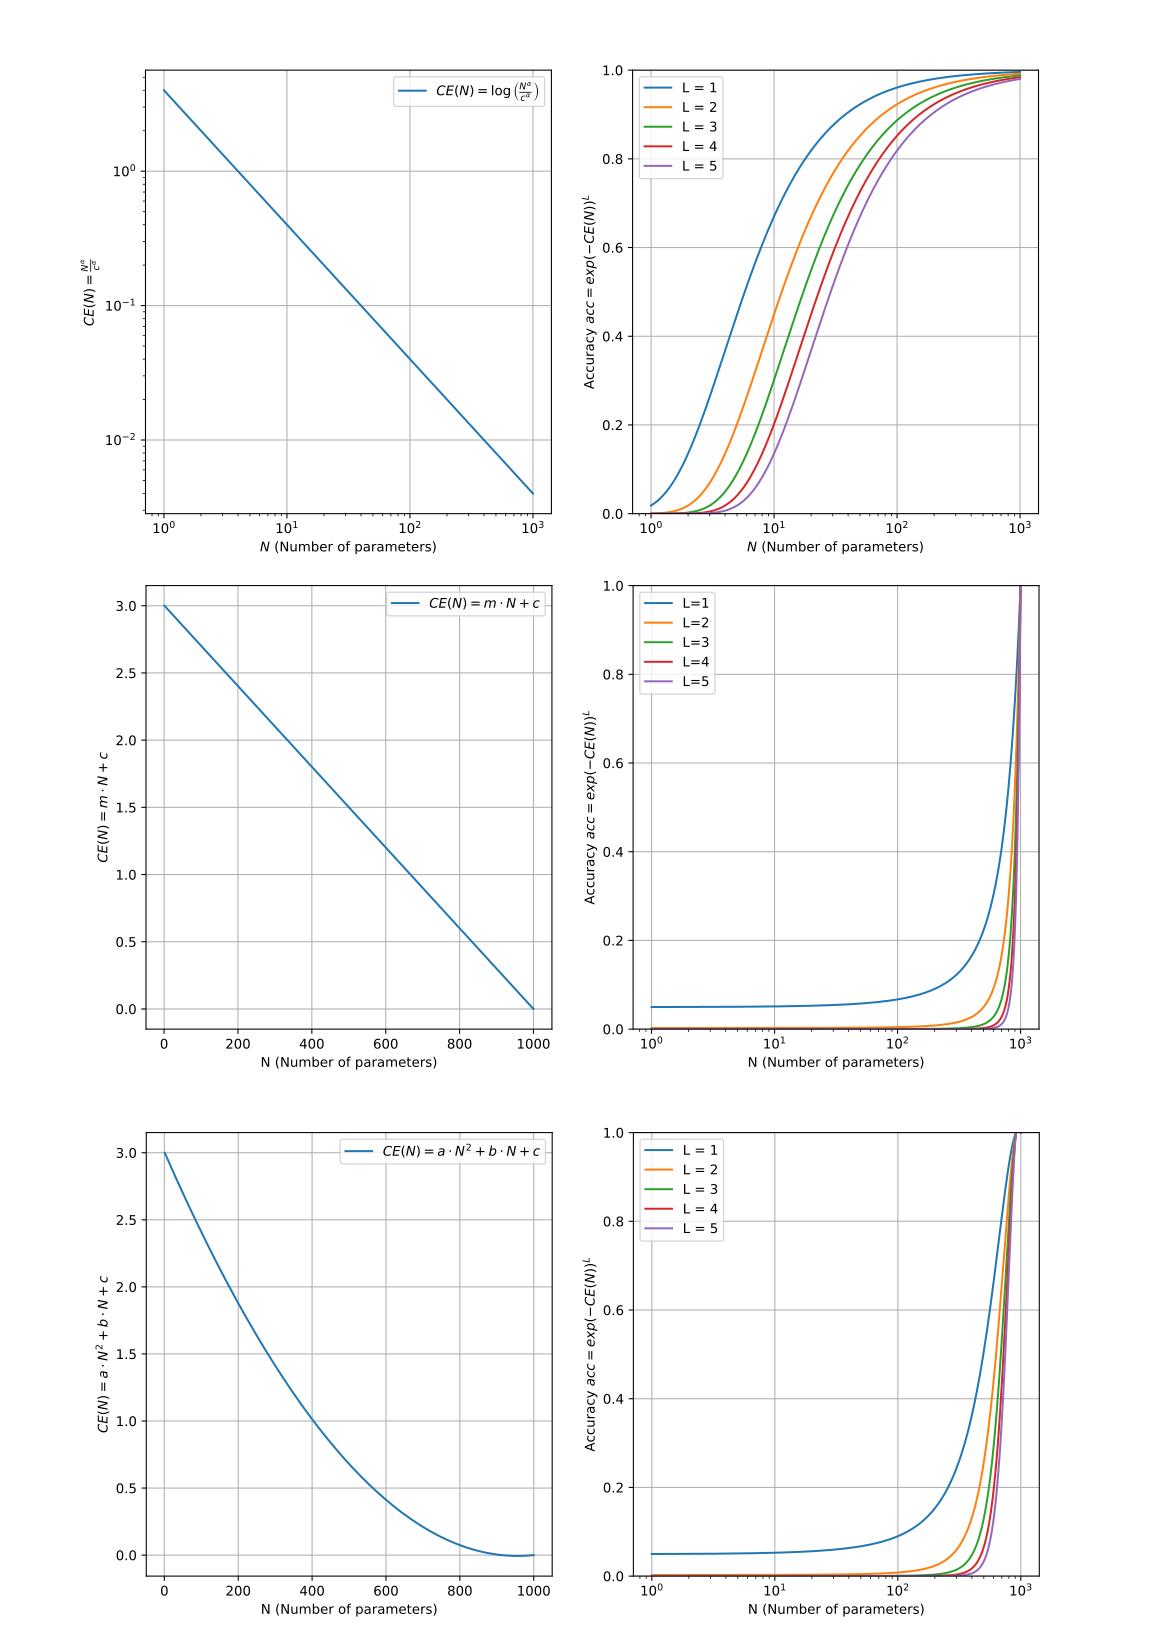
\includegraphics[width=0.8\textwidth]{figures/loss_decreasing_leads_to_emergence/decreasing_loss_leads_to_emergence_as_L_increases.png}
%   \caption{
%   \textbf{Emergence does not depend on scaling laws: any decreasing cross-entropy loss induces apparent emergence as L increases as you require more tokens to be exactly correct, i.e. L increases.}
%   The first row shows the same argument as in the main section, where a decreasing cross-entropy loss as a scaling law induces emergence as $L$ increases.
%   The second row shows the that apparent emergence is induced even when the cross-entropy loss decreases linearly.
%   The third row shows that the apparent emergence is induced when the cross-entropy loss decreases quadratically.
%   Emergence is amplified in this case especially by the increase in sharpness as more tokens are required to be correct. 
%   This means that simply changing the evaluation metric can suddenly induce emergence, and it is not an intrinsic property of the model. 
%   }
%   \label{fig:decreasing_loss_leads_to_emergence_as_L_increases}
% \end{figure}


\section{Inducing Emergent Abilities in Networks on Vision Tasks}
\label{app:sec:inducing_emergence_vision}

\subsection{Emergent Classification of MNIST Handwritten Digits by Convolutional Networks}

\begin{figure}
    \centering
    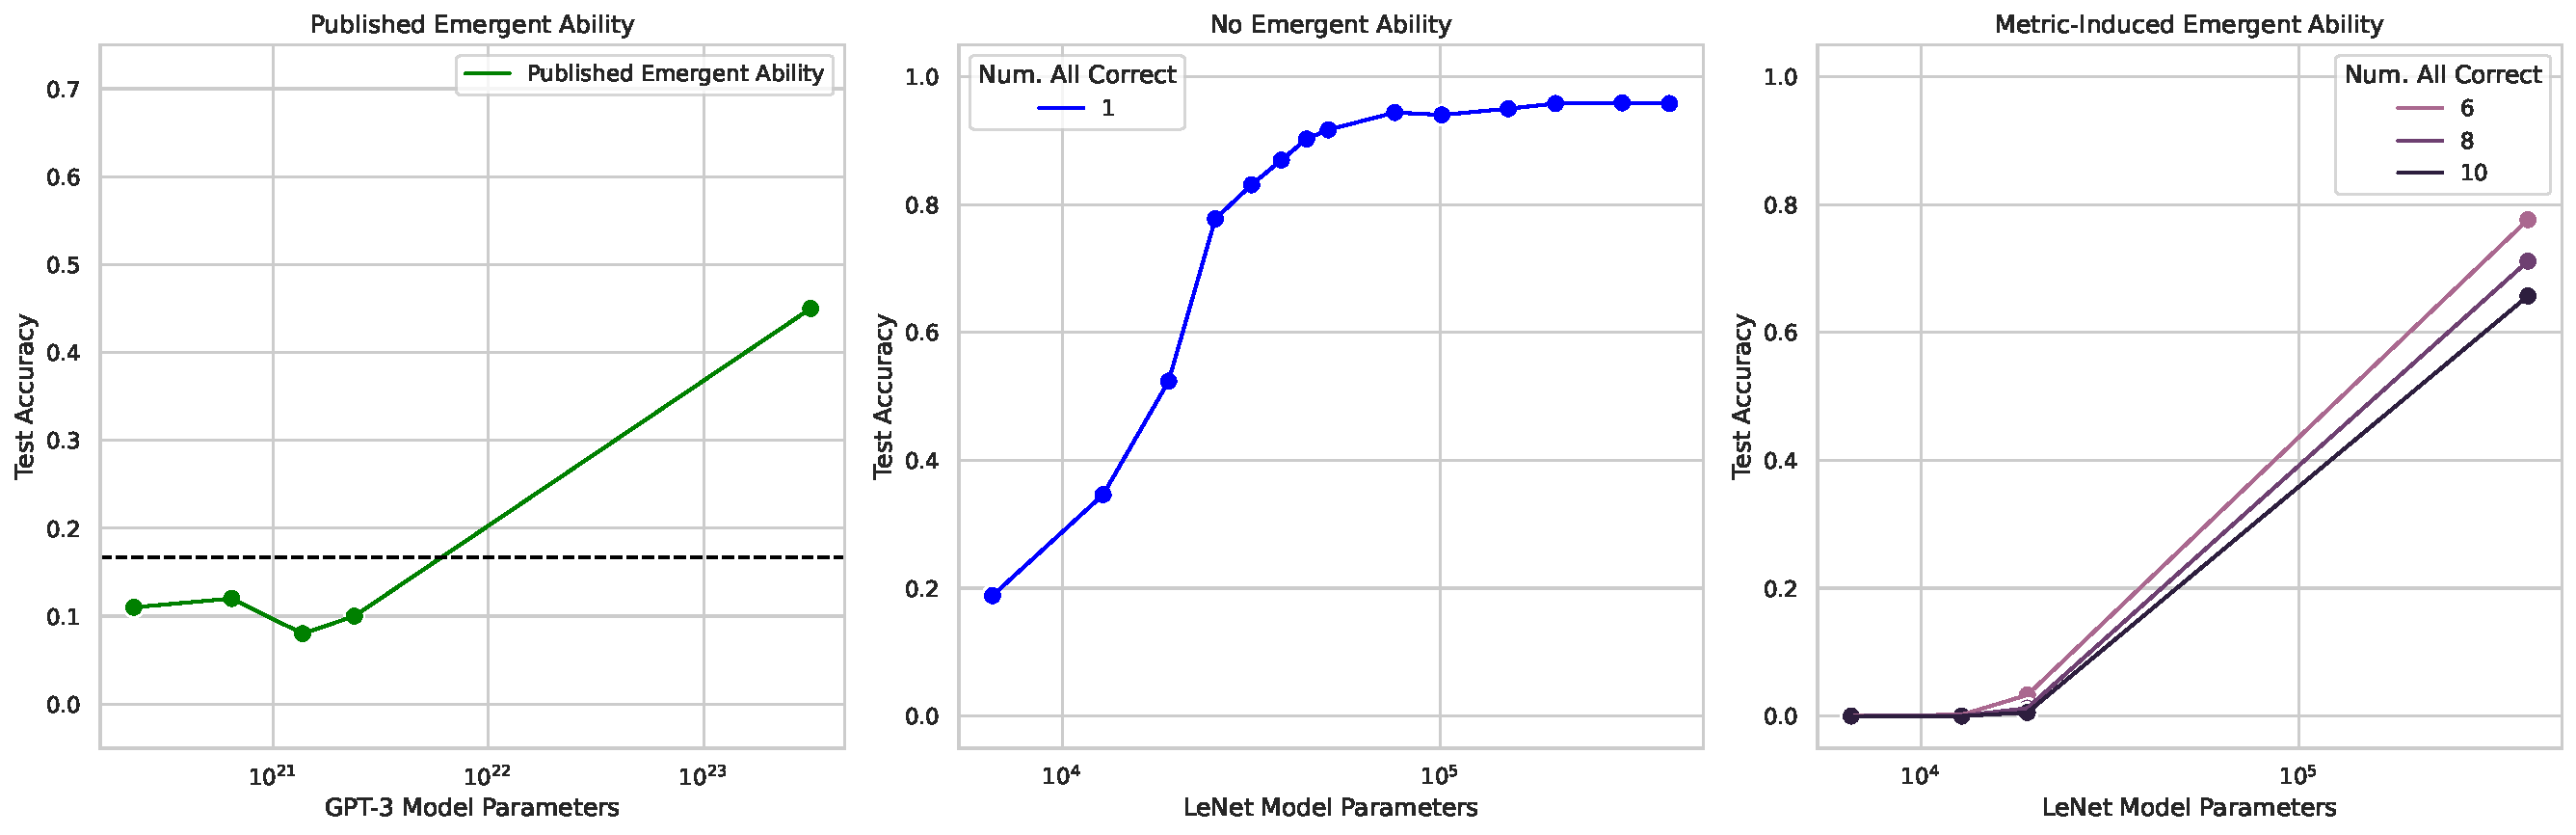
\includegraphics[width=\textwidth]{figures/vision/no_emergence_and_emergence_dataset=mnist.pdf}
    \caption{\textbf{Induced emergent MNIST classification ability in convolutional networks.} (A) A published emergent ability from the BIG-Bench Grounded Mappings task \cite{wei2022emergent}. (B) LeNet trained on MNIST \cite{lecun1998mnist} displays a predictable, commonplace sigmoidal increase in test accuracy as model parameters increase. (C) When accuracy is redefined as correctly classifying $K$ out of $K$ independent test data, this newly defined metric induces a seemingly unpredictable change.}
    \label{fig:vision_mnist}
\end{figure}

We begin by inducing an emergent classification ability in a LeNet convolutional neural network family \cite{lecun1998gradient}, trained on the MNIST handwritten digits dataset \cite{lecun1998mnist}.
This family displays smoothly increasing test accuracy as the number of parameters increase (Fig. \ref{fig:vision_mnist}B).
To emulate the accuracy metric used by emergence papers \cite{ganguli2022predictability, wei2022emergent, srivastava2022beyond}, we use \textit{subset accuracy}: 1 if the network classifies $K$ out of $K$ (independent) test data correctly, 0 otherwise.
Under this definition of accuracy, the model family displays an ``emergent" ability to correctly classify sets of MNIST digits as $K$ increases from $1$ to $5$, especially when combined with sparse sampling of model sizes (Fig. \ref{fig:vision_mnist}C).
This convolutional family's emergent classification ability qualitatively matches published emergent abilities, e.g., at the BIG-Bench Grounded Mappings task \cite{wei2022emergent} (Fig. \ref{fig:vision_mnist}A).


\end{document}
